\documentclass[twoside]{book}

% Packages required by doxygen
\usepackage{calc}
\usepackage{doxygen}
\usepackage{graphicx}
\usepackage[utf8]{inputenc}
\usepackage{makeidx}
\usepackage{multicol}
\usepackage{multirow}
\usepackage{textcomp}
\usepackage[table]{xcolor}

% Font selection
\usepackage[T1]{fontenc}
\usepackage{mathptmx}
\usepackage[scaled=.90]{helvet}
\usepackage{courier}
\usepackage{amssymb}
\usepackage{sectsty}
\renewcommand{\familydefault}{\sfdefault}
\allsectionsfont{%
  \fontseries{bc}\selectfont%
  \color{darkgray}%
}
\renewcommand{\DoxyLabelFont}{%
  \fontseries{bc}\selectfont%
  \color{darkgray}%
}

% Page & text layout
\usepackage{geometry}
\geometry{%
  a4paper,%
  top=2.5cm,%
  bottom=2.5cm,%
  left=2.5cm,%
  right=2.5cm%
}
\tolerance=750
\hfuzz=15pt
\hbadness=750
\setlength{\emergencystretch}{15pt}
\setlength{\parindent}{0cm}
\setlength{\parskip}{0.2cm}
\makeatletter
\renewcommand{\paragraph}{%
  \@startsection{paragraph}{4}{0ex}{-1.0ex}{1.0ex}{%
    \normalfont\normalsize\bfseries\SS@parafont%
  }%
}
\renewcommand{\subparagraph}{%
  \@startsection{subparagraph}{5}{0ex}{-1.0ex}{1.0ex}{%
    \normalfont\normalsize\bfseries\SS@subparafont%
  }%
}
\makeatother

% Headers & footers
\usepackage{fancyhdr}
\pagestyle{fancyplain}
\fancyhead[LE]{\fancyplain{}{\bfseries\thepage}}
\fancyhead[CE]{\fancyplain{}{}}
\fancyhead[RE]{\fancyplain{}{\bfseries\leftmark}}
\fancyhead[LO]{\fancyplain{}{\bfseries\rightmark}}
\fancyhead[CO]{\fancyplain{}{}}
\fancyhead[RO]{\fancyplain{}{\bfseries\thepage}}
\fancyfoot[LE]{\fancyplain{}{}}
\fancyfoot[CE]{\fancyplain{}{}}
\fancyfoot[RE]{\fancyplain{}{\bfseries\scriptsize Generated on Mon Nov 4 2013 14\-:37\-:30 for Log\-Viewer by Doxygen }}
\fancyfoot[LO]{\fancyplain{}{\bfseries\scriptsize Generated on Mon Nov 4 2013 14\-:37\-:30 for Log\-Viewer by Doxygen }}
\fancyfoot[CO]{\fancyplain{}{}}
\fancyfoot[RO]{\fancyplain{}{}}
\renewcommand{\footrulewidth}{0.4pt}
\renewcommand{\chaptermark}[1]{%
  \markboth{#1}{}%
}
\renewcommand{\sectionmark}[1]{%
  \markright{\thesection\ #1}%
}

% Indices & bibliography
\usepackage{natbib}
\usepackage[titles]{tocloft}
\setcounter{tocdepth}{3}
\setcounter{secnumdepth}{5}
\makeindex

% Hyperlinks (required, but should be loaded last)
\usepackage{ifpdf}
\ifpdf
  \usepackage[pdftex,pagebackref=true]{hyperref}
\else
  \usepackage[ps2pdf,pagebackref=true]{hyperref}
\fi
\hypersetup{%
  colorlinks=true,%
  linkcolor=blue,%
  citecolor=blue,%
  unicode%
}

% Custom commands
\newcommand{\clearemptydoublepage}{%
  \newpage{\pagestyle{empty}\cleardoublepage}%
}


%===== C O N T E N T S =====

\begin{document}

% Titlepage & ToC
\hypersetup{pageanchor=false}
\pagenumbering{roman}
\begin{titlepage}
\vspace*{7cm}
\begin{center}%
{\Large Log\-Viewer }\\
\vspace*{1cm}
{\large Generated by Doxygen 1.8.5}\\
\vspace*{0.5cm}
{\small Mon Nov 4 2013 14:37:30}\\
\end{center}
\end{titlepage}
\clearemptydoublepage
\tableofcontents
\clearemptydoublepage
\pagenumbering{arabic}
\hypersetup{pageanchor=true}

%--- Begin generated contents ---
\chapter{Main Page}
\label{index}\hypertarget{index}{}Log\-Viewer is developed to be able to quickly view and analyze log files or content from online log clients.

\begin{DoxyNote}{Note}
A lot of emphasis has been put on providing a compelling look-\/and-\/feel to the application and to give the user a feeling of not feeling stupid using the application.

One way of doing this is to provide more than one way of doing common tasks such as opening a log file, for example use short-\/cut, menu, toolbar, drag n' drop etc.

Another way is to never popup any dialogs that informs the user that a entered value is out of range or prompts for input. Also make sure to disable all buttons and menus that the end user currently can't use. For example, if the filter input edit is empty the apply filer button is disabled, if the user starts to type the button is enabled. Use placeholder\-Text in all edit fields to inform what's supposed to be entered. Example\-: the filter input has the placeholder\-Text set to \char`\"{}\-Enter text to filter\char`\"{}.
\end{DoxyNote}
{\bfseries  The documentation is intended to aid developers of the application, not to provide a user guide to the end-\/user. }

The following sections are describing the implementation in more detail\-:
\begin{DoxyItemize}
\item \hyperlink{_g_u_i}{The G\-U\-I}
\item \hyperlink{_log_manager}{The manager}.
\item \hyperlink{_log_formats}{Log Formats}
\end{DoxyItemize}

A goal has been to follow the J\-S\-F Coding Standard (link\-: \hyperlink{}{http\-://www2.\-research.\-att.\-com/$\sim$bs/\-J\-S\-F-\/\-A\-V-\/rules.\-pdf}).

\begin{DoxyAuthor}{Author}
Tommy Gustavsson 
\end{DoxyAuthor}
\begin{DoxyVersion}{Version}
0.\-x 
\end{DoxyVersion}

\chapter{The G\-U\-I}
\label{_g_u_i}
\hypertarget{_g_u_i}{}
The G\-U\-I is composed in the Main\-\_\-window class. No application logic shall be present in the Main\-\_\-window class, all application logic must be separated from the presentation. Use S\-I\-G\-N\-A\-L, S\-L\-O\-T, models etc. to accomplish this. 
\chapter{The manager}
\label{_log_manager}
\hypertarget{_log_manager}{}
The \hyperlink{class_log__viewer_1_1_log__manager}{Log\-\_\-manager} puts together the different parts of business logic that ends up acting like an application. The G\-U\-I part is only a visualization of this class.

There are four models that provide access to data\-:
\begin{DoxyItemize}
\item \hyperlink{class_log__viewer_1_1_log__items__model}{Log\-\_\-items\-\_\-model}\-: This model contains all log entries and defines the behaviour of such things as color typing, columns, text highlight.
\item \hyperlink{class_log__viewer_1_1_log__filter__proxy__model}{Log\-\_\-filter\-\_\-proxy\-\_\-model}\-: This model is placed inbetween the Q\-Table\-View and the \hyperlink{class_log__viewer_1_1_log__items__model}{Log\-\_\-items\-\_\-model} to provide filtering. 
\begin{DoxyCode}
m\_log\_filter\_proxy\_model->setSourceModel(m\_log\_items\_model);
\end{DoxyCode}

\item \hyperlink{class_log__viewer_1_1_clients__model}{Clients\-\_\-model}\-: This model holds the set of connected \hyperlink{class_log__viewer_1_1_log__client}{Log\-\_\-clients}.
\item \hyperlink{class_log__viewer_1_1_file__neighbor__model}{File\-\_\-neighbor\-\_\-model}\-: This models contains all files that are in the same folder as the last opened file.
\end{DoxyItemize}

These models is accessable from the \hyperlink{class_log__viewer_1_1_log__manager}{Log\-\_\-manager} class. 
\begin{DoxyCode}
Log\_items\_model* log\_items\_model()\textcolor{keyword}{ const }\{
    \textcolor{keywordflow}{return} m\_log\_items\_model;
\}

Clients\_model* clients\_model()\textcolor{keyword}{ const }\{
    \textcolor{keywordflow}{return} m\_clients\_model;
\}

Log\_filter\_proxy\_model* log\_filter\_proxy\_model()\textcolor{keyword}{ const }\{
    \textcolor{keywordflow}{return} m\_log\_filter\_proxy\_model;
\}

File\_neighbor\_model* file\_neighbor\_model()\textcolor{keyword}{ const }\{
    \textcolor{keywordflow}{return} m\_file\_neighbor\_model;
\}
\end{DoxyCode}


The \hyperlink{class_log__viewer_1_1_log__manager}{Log\-\_\-manager} is accessed through a \hyperlink{class_singleton}{singleton}. 
\begin{DoxyCode}
Log\_manager::instance->file\_neighbor\_model()
\end{DoxyCode}


The \hyperlink{class_log__viewer_1_1_log__manager}{Log\-\_\-manager} does not create any threads. Thread safety has not been the focus so far, perhaps this will need to be addressed. There are several operations that potentially can take a lot of time, such as filtering, highlightning, loading from file etc. With the current design the application will need to wait \char`\"{}freeze\char`\"{} until the operations has finished. 
\chapter{Log Formats}
\label{_log_formats}
\hypertarget{_log_formats}{}
A log format is defined as a line of text where its data is separated by a single char or a string. The log format can also have a specific start and stop sequence to indicate start and end of text, this is especially good when using it over the network.

\hyperlink{class_log__viewer_1_1_log__format}{Log\-\_\-format} is the interface for all inherited formats, override the pure virtual functions to implement a new format\-: 
\begin{DoxyCode}
\textcolor{keyword}{public}:
    \textcolor{keyword}{virtual} QString get\_description() \textcolor{keyword}{const} = 0;
    \textcolor{keyword}{virtual} QString get\_start\_seq() \textcolor{keyword}{const} = 0;
    \textcolor{keyword}{virtual} QString get\_stop\_seq() \textcolor{keyword}{const} = 0;
    \textcolor{keyword}{virtual} QString get\_origin() \textcolor{keyword}{const} = 0;
    \textcolor{keyword}{virtual} \textcolor{keywordtype}{bool} match(\textcolor{keyword}{const} QString first\_line) \textcolor{keyword}{const} = 0;
\textcolor{keyword}{private}:
    \textcolor{keyword}{virtual} QSharedPointer<Log\_item> create\_log\_item(\textcolor{keyword}{const} QString value, \textcolor{keyword}{const} QString origin) \textcolor{keyword}{const} = 0;
\end{DoxyCode}


As seen above a \hyperlink{class_log__viewer_1_1_log__format}{Log\-\_\-format} class decendant is responsible for the creation of its log items.

\hyperlink{class_log__viewer_1_1_log__item}{Log\-\_\-item} serves as the base class for log items. A log item is used to break down the line of text to its predefined data structure. The data structure will eventually end up as columns in the G\-U\-I. This is a list of the data structure, all access to these private variables is done with a getter. 
\begin{DoxyCode}
\textcolor{keywordtype}{int} m\_index;
Log\_type m\_type;
QString m\_text;
QString m\_date;
QString m\_time;
QString m\_file;
QString m\_line;
QString m\_application;
QString m\_module;
QString m\_thread;
QString m\_origin;
\end{DoxyCode}


In the name of simplicity for the end user all formats shall try to auto-\/sense its format when requested. To ensure a valid match regular expressions are used. 
\begin{DoxyCode}
\textcolor{keyword}{virtual} \textcolor{keywordtype}{bool} match(\textcolor{keyword}{const} QString first\_line) \textcolor{keyword}{const} = 0;
\end{DoxyCode}
 As an improvemnet the formats could be loaded on demand via Q\-T plugin architecture.

To add a format you need to modify the \hyperlink{class_log__viewer_1_1_log__format__factory}{Log\-\_\-format\-\_\-factor} class. 
\begin{DoxyCode}
QSharedPointer<Log\_format> Log\_format\_factory::create(\textcolor{keyword}{const} QString first\_line, \textcolor{keyword}{const} QString origin)
\{
    QSharedPointer<Log\_format> format;

    format = QSharedPointer<G3\_log\_format>(\textcolor{keyword}{new} G3\_log\_format(origin));
    \textcolor{keywordflow}{if}(format->match(first\_line))
        \textcolor{keywordflow}{return} format;

    format = QSharedPointer<NRG\_log\_format>(\textcolor{keyword}{new} NRG\_log\_format(origin));
    \textcolor{keywordflow}{if}(format->match(first\_line))
        \textcolor{keywordflow}{return} format;

    format = QSharedPointer<NRG\_legacy\_log\_format>(\textcolor{keyword}{new} NRG\_legacy\_log\_format(origin));
    \textcolor{keywordflow}{if}(format->match(first\_line))
        \textcolor{keywordflow}{return} format;

    \textcolor{comment}{// Add new format here...}

    \textcolor{keywordflow}{return} QSharedPointer<Unknown\_log\_format>(\textcolor{keyword}{new} Unknown\_log\_format());
\}
\end{DoxyCode}
 
\chapter{Hierarchical Index}
\section{Class Hierarchy}
This inheritance list is sorted roughly, but not completely, alphabetically\-:\begin{DoxyCompactList}
\item \contentsline{section}{Color\-\_\-theme}{\pageref{struct_color__theme}}{}
\item \contentsline{section}{Log\-\_\-viewer\-:\-:Log\-\_\-column}{\pageref{struct_log__viewer_1_1_log__column}}{}
\item \contentsline{section}{Log\-\_\-viewer\-:\-:Log\-\_\-format\-\_\-factory}{\pageref{class_log__viewer_1_1_log__format__factory}}{}
\item \contentsline{section}{Log\-\_\-viewer\-:\-:Log\-\_\-item}{\pageref{class_log__viewer_1_1_log__item}}{}
\begin{DoxyCompactList}
\item \contentsline{section}{Log\-\_\-viewer\-:\-:App\-\_\-log\-\_\-item}{\pageref{class_log__viewer_1_1_app__log__item}}{}
\item \contentsline{section}{Log\-\_\-viewer\-:\-:G3\-\_\-log\-\_\-item}{\pageref{class_log__viewer_1_1_g3__log__item}}{}
\item \contentsline{section}{Log\-\_\-viewer\-:\-:N\-R\-G\-\_\-legacy\-\_\-log\-\_\-item}{\pageref{class_log__viewer_1_1_n_r_g__legacy__log__item}}{}
\item \contentsline{section}{Log\-\_\-viewer\-:\-:N\-R\-G\-\_\-log\-\_\-item}{\pageref{class_log__viewer_1_1_n_r_g__log__item}}{}
\item \contentsline{section}{Log\-\_\-viewer\-:\-:Plain\-\_\-text\-\_\-log\-\_\-item}{\pageref{class_log__viewer_1_1_plain__text__log__item}}{}
\end{DoxyCompactList}
\item Q\-Abstract\-List\-Model\begin{DoxyCompactList}
\item \contentsline{section}{Log\-\_\-viewer\-:\-:Clients\-\_\-model}{\pageref{class_log__viewer_1_1_clients__model}}{}
\item \contentsline{section}{Log\-\_\-viewer\-:\-:File\-\_\-neighbor\-\_\-model}{\pageref{class_log__viewer_1_1_file__neighbor__model}}{}
\item \contentsline{section}{Log\-\_\-viewer\-:\-:ftp\-\_\-files\-\_\-model}{\pageref{class_log__viewer_1_1ftp__files__model}}{}
\end{DoxyCompactList}
\item Q\-Abstract\-Table\-Model\begin{DoxyCompactList}
\item \contentsline{section}{Log\-\_\-viewer\-:\-:Log\-\_\-items\-\_\-model}{\pageref{class_log__viewer_1_1_log__items__model}}{}
\end{DoxyCompactList}
\item Q\-Frame\begin{DoxyCompactList}
\item \contentsline{section}{Colored\-\_\-frame}{\pageref{class_colored__frame}}{}
\end{DoxyCompactList}
\item Q\-Main\-Window\begin{DoxyCompactList}
\item \contentsline{section}{Main\-\_\-window}{\pageref{class_main__window}}{}
\end{DoxyCompactList}
\item Q\-Object\begin{DoxyCompactList}
\item \contentsline{section}{Log\-\_\-viewer\-:\-:Log\-\_\-client}{\pageref{class_log__viewer_1_1_log__client}}{}
\item \contentsline{section}{Log\-\_\-viewer\-:\-:Log\-\_\-file\-\_\-parser}{\pageref{class_log__viewer_1_1_log__file__parser}}{}
\item \contentsline{section}{Log\-\_\-viewer\-:\-:Log\-\_\-format}{\pageref{class_log__viewer_1_1_log__format}}{}
\begin{DoxyCompactList}
\item \contentsline{section}{Log\-\_\-viewer\-:\-:G3\-\_\-log\-\_\-format}{\pageref{class_log__viewer_1_1_g3__log__format}}{}
\item \contentsline{section}{Log\-\_\-viewer\-:\-:N\-R\-G\-\_\-legacy\-\_\-log\-\_\-format}{\pageref{struct_log__viewer_1_1_n_r_g__legacy__log__format}}{}
\item \contentsline{section}{Log\-\_\-viewer\-:\-:N\-R\-G\-\_\-log\-\_\-format}{\pageref{struct_log__viewer_1_1_n_r_g__log__format}}{}
\item \contentsline{section}{Log\-\_\-viewer\-:\-:Unknown\-\_\-log\-\_\-format}{\pageref{struct_log__viewer_1_1_unknown__log__format}}{}
\end{DoxyCompactList}
\item \contentsline{section}{Log\-\_\-viewer\-:\-:Log\-\_\-manager}{\pageref{class_log__viewer_1_1_log__manager}}{}
\item \contentsline{section}{Log\-\_\-viewer\-:\-:Start\-\_\-stop\-\_\-buffer}{\pageref{class_log__viewer_1_1_start__stop__buffer}}{}
\item \contentsline{section}{Log\-\_\-viewer\-:\-:Tail}{\pageref{class_log__viewer_1_1_tail}}{}
\end{DoxyCompactList}
\item Q\-Sort\-Filter\-Proxy\-Model\begin{DoxyCompactList}
\item \contentsline{section}{Log\-\_\-viewer\-:\-:Log\-\_\-filter\-\_\-proxy\-\_\-model}{\pageref{class_log__viewer_1_1_log__filter__proxy__model}}{}
\end{DoxyCompactList}
\item Q\-Table\-View\begin{DoxyCompactList}
\item \contentsline{section}{Log\-\_\-table\-\_\-view}{\pageref{class_log__table__view}}{}
\end{DoxyCompactList}
\item Q\-Text\-Edit\begin{DoxyCompactList}
\item \contentsline{section}{Log\-\_\-item\-\_\-preview\-\_\-text\-Edit}{\pageref{class_log__item__preview__text_edit}}{}
\end{DoxyCompactList}
\item \contentsline{section}{Singleton$<$ T $>$}{\pageref{class_singleton}}{}
\end{DoxyCompactList}

\chapter{Class Index}
\section{Class List}
Here are the classes, structs, unions and interfaces with brief descriptions\-:\begin{DoxyCompactList}
\item\contentsline{section}{\hyperlink{class_log__viewer_1_1_app__log__item}{Log\-\_\-viewer\-::\-App\-\_\-log\-\_\-item} }{\pageref{class_log__viewer_1_1_app__log__item}}{}
\item\contentsline{section}{\hyperlink{class_log__viewer_1_1_clients__model}{Log\-\_\-viewer\-::\-Clients\-\_\-model} }{\pageref{class_log__viewer_1_1_clients__model}}{}
\item\contentsline{section}{\hyperlink{struct_color__theme}{Color\-\_\-theme} }{\pageref{struct_color__theme}}{}
\item\contentsline{section}{\hyperlink{class_colored__frame}{Colored\-\_\-frame} }{\pageref{class_colored__frame}}{}
\item\contentsline{section}{\hyperlink{class_log__viewer_1_1_file__neighbor__model}{Log\-\_\-viewer\-::\-File\-\_\-neighbor\-\_\-model} }{\pageref{class_log__viewer_1_1_file__neighbor__model}}{}
\item\contentsline{section}{\hyperlink{class_log__viewer_1_1ftp__files__model}{Log\-\_\-viewer\-::ftp\-\_\-files\-\_\-model} }{\pageref{class_log__viewer_1_1ftp__files__model}}{}
\item\contentsline{section}{\hyperlink{class_log__viewer_1_1_g3__log__format}{Log\-\_\-viewer\-::\-G3\-\_\-log\-\_\-format} }{\pageref{class_log__viewer_1_1_g3__log__format}}{}
\item\contentsline{section}{\hyperlink{class_log__viewer_1_1_g3__log__item}{Log\-\_\-viewer\-::\-G3\-\_\-log\-\_\-item} }{\pageref{class_log__viewer_1_1_g3__log__item}}{}
\item\contentsline{section}{\hyperlink{class_log__viewer_1_1_log__client}{Log\-\_\-viewer\-::\-Log\-\_\-client} }{\pageref{class_log__viewer_1_1_log__client}}{}
\item\contentsline{section}{\hyperlink{struct_log__viewer_1_1_log__column}{Log\-\_\-viewer\-::\-Log\-\_\-column} }{\pageref{struct_log__viewer_1_1_log__column}}{}
\item\contentsline{section}{\hyperlink{class_log__viewer_1_1_log__file__parser}{Log\-\_\-viewer\-::\-Log\-\_\-file\-\_\-parser} }{\pageref{class_log__viewer_1_1_log__file__parser}}{}
\item\contentsline{section}{\hyperlink{class_log__viewer_1_1_log__filter__proxy__model}{Log\-\_\-viewer\-::\-Log\-\_\-filter\-\_\-proxy\-\_\-model} }{\pageref{class_log__viewer_1_1_log__filter__proxy__model}}{}
\item\contentsline{section}{\hyperlink{class_log__viewer_1_1_log__format}{Log\-\_\-viewer\-::\-Log\-\_\-format} }{\pageref{class_log__viewer_1_1_log__format}}{}
\item\contentsline{section}{\hyperlink{class_log__viewer_1_1_log__format__factory}{Log\-\_\-viewer\-::\-Log\-\_\-format\-\_\-factory} }{\pageref{class_log__viewer_1_1_log__format__factory}}{}
\item\contentsline{section}{\hyperlink{class_log__viewer_1_1_log__item}{Log\-\_\-viewer\-::\-Log\-\_\-item} }{\pageref{class_log__viewer_1_1_log__item}}{}
\item\contentsline{section}{\hyperlink{class_log__item__preview__text_edit}{Log\-\_\-item\-\_\-preview\-\_\-text\-Edit} }{\pageref{class_log__item__preview__text_edit}}{}
\item\contentsline{section}{\hyperlink{class_log__viewer_1_1_log__items__model}{Log\-\_\-viewer\-::\-Log\-\_\-items\-\_\-model} }{\pageref{class_log__viewer_1_1_log__items__model}}{}
\item\contentsline{section}{\hyperlink{class_log__viewer_1_1_log__manager}{Log\-\_\-viewer\-::\-Log\-\_\-manager} }{\pageref{class_log__viewer_1_1_log__manager}}{}
\item\contentsline{section}{\hyperlink{class_log__table__view}{Log\-\_\-table\-\_\-view} }{\pageref{class_log__table__view}}{}
\item\contentsline{section}{\hyperlink{class_main__window}{Main\-\_\-window} }{\pageref{class_main__window}}{}
\item\contentsline{section}{\hyperlink{struct_log__viewer_1_1_n_r_g__legacy__log__format}{Log\-\_\-viewer\-::\-N\-R\-G\-\_\-legacy\-\_\-log\-\_\-format} }{\pageref{struct_log__viewer_1_1_n_r_g__legacy__log__format}}{}
\item\contentsline{section}{\hyperlink{class_log__viewer_1_1_n_r_g__legacy__log__item}{Log\-\_\-viewer\-::\-N\-R\-G\-\_\-legacy\-\_\-log\-\_\-item} }{\pageref{class_log__viewer_1_1_n_r_g__legacy__log__item}}{}
\item\contentsline{section}{\hyperlink{struct_log__viewer_1_1_n_r_g__log__format}{Log\-\_\-viewer\-::\-N\-R\-G\-\_\-log\-\_\-format} }{\pageref{struct_log__viewer_1_1_n_r_g__log__format}}{}
\item\contentsline{section}{\hyperlink{class_log__viewer_1_1_n_r_g__log__item}{Log\-\_\-viewer\-::\-N\-R\-G\-\_\-log\-\_\-item} }{\pageref{class_log__viewer_1_1_n_r_g__log__item}}{}
\item\contentsline{section}{\hyperlink{class_log__viewer_1_1_plain__text__log__item}{Log\-\_\-viewer\-::\-Plain\-\_\-text\-\_\-log\-\_\-item} }{\pageref{class_log__viewer_1_1_plain__text__log__item}}{}
\item\contentsline{section}{\hyperlink{class_singleton}{Singleton$<$ T $>$} }{\pageref{class_singleton}}{}
\item\contentsline{section}{\hyperlink{class_log__viewer_1_1_start__stop__buffer}{Log\-\_\-viewer\-::\-Start\-\_\-stop\-\_\-buffer} }{\pageref{class_log__viewer_1_1_start__stop__buffer}}{}
\item\contentsline{section}{\hyperlink{class_log__viewer_1_1_tail}{Log\-\_\-viewer\-::\-Tail} }{\pageref{class_log__viewer_1_1_tail}}{}
\item\contentsline{section}{\hyperlink{struct_log__viewer_1_1_unknown__log__format}{Log\-\_\-viewer\-::\-Unknown\-\_\-log\-\_\-format} }{\pageref{struct_log__viewer_1_1_unknown__log__format}}{}
\end{DoxyCompactList}

\chapter{Class Documentation}
\hypertarget{class_log__viewer_1_1_app__log__item}{\section{Log\-\_\-viewer\-:\-:App\-\_\-log\-\_\-item Class Reference}
\label{class_log__viewer_1_1_app__log__item}\index{Log\-\_\-viewer\-::\-App\-\_\-log\-\_\-item@{Log\-\_\-viewer\-::\-App\-\_\-log\-\_\-item}}
}
Inheritance diagram for Log\-\_\-viewer\-:\-:App\-\_\-log\-\_\-item\-:\begin{figure}[H]
\begin{center}
\leavevmode
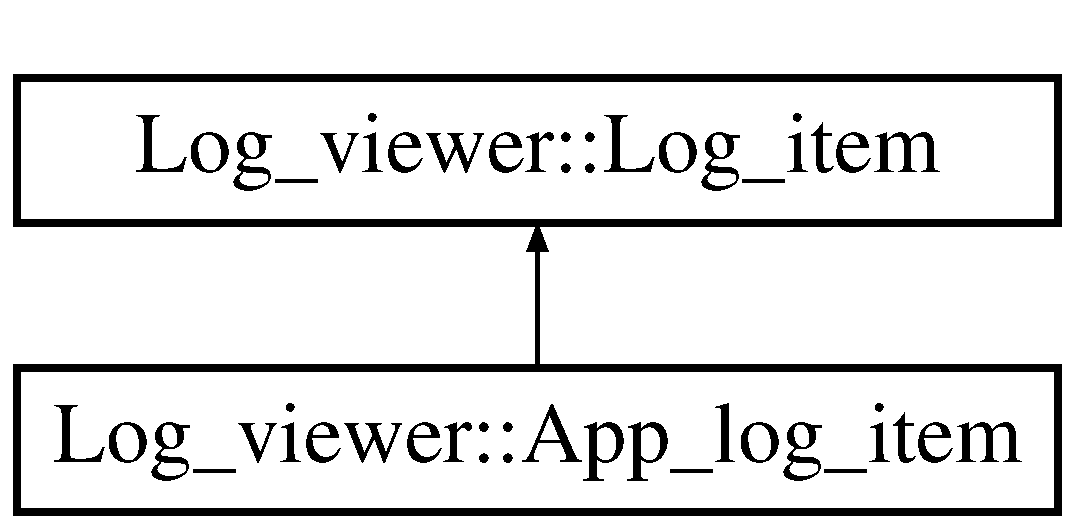
\includegraphics[height=2.000000cm]{class_log__viewer_1_1_app__log__item}
\end{center}
\end{figure}
\subsection*{Public Member Functions}
\begin{DoxyCompactItemize}
\item 
\hypertarget{class_log__viewer_1_1_app__log__item_afb5eeaf3f20fbaa8eb959f956c99f946}{{\bfseries App\-\_\-log\-\_\-item} (const Q\-String value, const Q\-String separator, const Q\-String origin)}\label{class_log__viewer_1_1_app__log__item_afb5eeaf3f20fbaa8eb959f956c99f946}

\end{DoxyCompactItemize}
\subsection*{Protected Member Functions}
\begin{DoxyCompactItemize}
\item 
\hypertarget{class_log__viewer_1_1_app__log__item_ace8a51aab56a113d1b7ffcb093bc7ec7}{Log\-\_\-type {\bfseries Log\-\_\-type\-\_\-from\-\_\-string} (const Q\-String value)}\label{class_log__viewer_1_1_app__log__item_ace8a51aab56a113d1b7ffcb093bc7ec7}

\end{DoxyCompactItemize}
\subsection*{Additional Inherited Members}


The documentation for this class was generated from the following files\-:\begin{DoxyCompactItemize}
\item 
app\-\_\-log\-\_\-item.\-h\item 
app\-\_\-log\-\_\-item.\-cpp\end{DoxyCompactItemize}

\hypertarget{class_log__viewer_1_1_clients__model}{\section{Log\-\_\-viewer\-:\-:Clients\-\_\-model Class Reference}
\label{class_log__viewer_1_1_clients__model}\index{Log\-\_\-viewer\-::\-Clients\-\_\-model@{Log\-\_\-viewer\-::\-Clients\-\_\-model}}
}
Inheritance diagram for Log\-\_\-viewer\-:\-:Clients\-\_\-model\-:\begin{figure}[H]
\begin{center}
\leavevmode
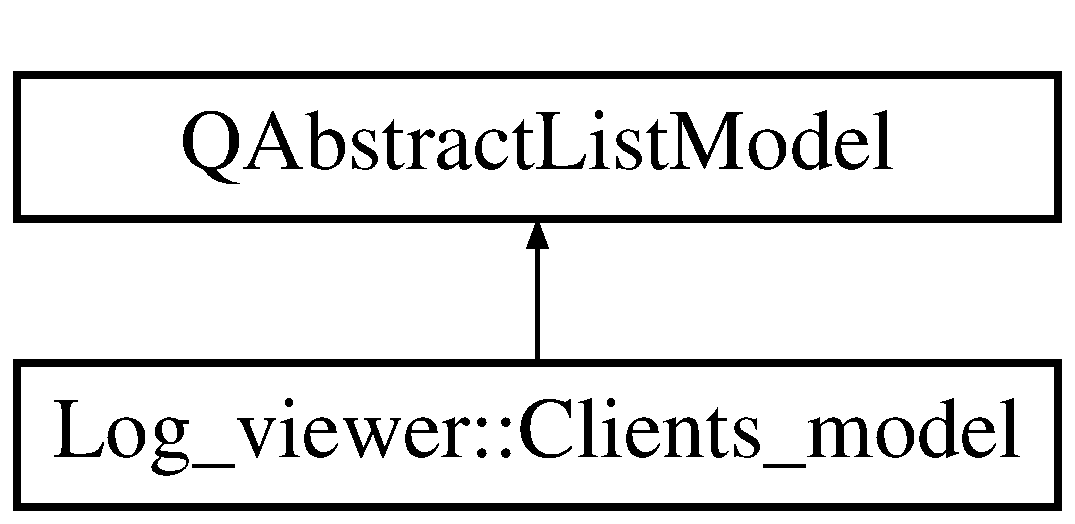
\includegraphics[height=2.000000cm]{class_log__viewer_1_1_clients__model}
\end{center}
\end{figure}
\subsection*{Public Member Functions}
\begin{DoxyCompactItemize}
\item 
\hypertarget{class_log__viewer_1_1_clients__model_ae3025cde857940ca06774f26f2427b9e}{{\bfseries Clients\-\_\-model} (Q\-Object $\ast$parent=0)}\label{class_log__viewer_1_1_clients__model_ae3025cde857940ca06774f26f2427b9e}

\item 
\hypertarget{class_log__viewer_1_1_clients__model_a27cd1770bc0a7725a562cc2d4ca25885}{int {\bfseries row\-Count} (const Q\-Model\-Index \&parent) const }\label{class_log__viewer_1_1_clients__model_a27cd1770bc0a7725a562cc2d4ca25885}

\item 
\hypertarget{class_log__viewer_1_1_clients__model_a59e88ce800e5fa1a717a01c2d90ece2d}{Q\-Variant {\bfseries data} (const Q\-Model\-Index \&index, int role) const }\label{class_log__viewer_1_1_clients__model_a59e88ce800e5fa1a717a01c2d90ece2d}

\item 
\hypertarget{class_log__viewer_1_1_clients__model_a8ab5e0f6ee051524bb5ce1f3f817eb2f}{void {\bfseries add} (Q\-Shared\-Pointer$<$ \hyperlink{class_log__viewer_1_1_log__client}{Log\-\_\-client} $>$ client)}\label{class_log__viewer_1_1_clients__model_a8ab5e0f6ee051524bb5ce1f3f817eb2f}

\item 
\hypertarget{class_log__viewer_1_1_clients__model_a4b683752dfac654431cd0b7f29d1029a}{void {\bfseries remove} (const \hyperlink{class_log__viewer_1_1_log__client}{Log\-\_\-client} $\ast$client)}\label{class_log__viewer_1_1_clients__model_a4b683752dfac654431cd0b7f29d1029a}

\item 
\hypertarget{class_log__viewer_1_1_clients__model_a7b2e3e695ff7af23551615a1872b544c}{void {\bfseries clear} ()}\label{class_log__viewer_1_1_clients__model_a7b2e3e695ff7af23551615a1872b544c}

\end{DoxyCompactItemize}


The documentation for this class was generated from the following files\-:\begin{DoxyCompactItemize}
\item 
clients\-\_\-model.\-h\item 
clients\-\_\-model.\-cpp\end{DoxyCompactItemize}

\hypertarget{struct_color__theme}{\section{Color\-\_\-theme Struct Reference}
\label{struct_color__theme}\index{Color\-\_\-theme@{Color\-\_\-theme}}
}
\subsection*{Public Member Functions}
\begin{DoxyCompactItemize}
\item 
\hypertarget{struct_color__theme_ad7958bf1cce7b96eb8c8726390a8b510}{{\bfseries Color\-\_\-theme} (const Q\-Color array\mbox{[}5\mbox{]})}\label{struct_color__theme_ad7958bf1cce7b96eb8c8726390a8b510}

\end{DoxyCompactItemize}
\subsection*{Public Attributes}
\begin{DoxyCompactItemize}
\item 
\hypertarget{struct_color__theme_ab5a1de0f04224abfe2942e614c2657b1}{Q\-Color {\bfseries c} \mbox{[}5\mbox{]}}\label{struct_color__theme_ab5a1de0f04224abfe2942e614c2657b1}

\item 
\hypertarget{struct_color__theme_a008de361633246354c382c2285e031de}{Q\-String {\bfseries name}}\label{struct_color__theme_a008de361633246354c382c2285e031de}

\end{DoxyCompactItemize}


The documentation for this struct was generated from the following files\-:\begin{DoxyCompactItemize}
\item 
color\-\_\-theme.\-h\item 
color\-\_\-theme.\-cpp\end{DoxyCompactItemize}

\hypertarget{class_colored__frame}{\section{Colored\-\_\-frame Class Reference}
\label{class_colored__frame}\index{Colored\-\_\-frame@{Colored\-\_\-frame}}
}
Inheritance diagram for Colored\-\_\-frame\-:\begin{figure}[H]
\begin{center}
\leavevmode
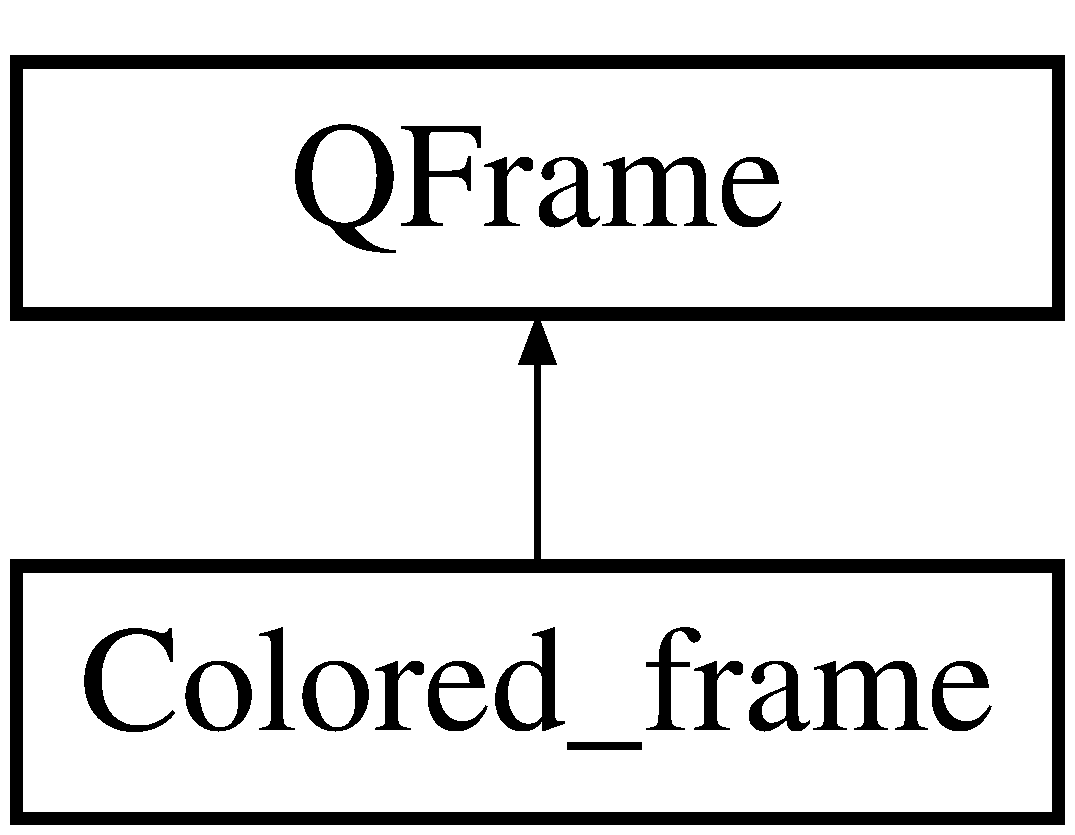
\includegraphics[height=2.000000cm]{class_colored__frame}
\end{center}
\end{figure}
\subsection*{Signals}
\begin{DoxyCompactItemize}
\item 
\hypertarget{class_colored__frame_a6cda11e629446453b6fb82713dd0f90c}{void {\bfseries context\-\_\-menu\-\_\-event} (Q\-Context\-Menu\-Event $\ast$event)}\label{class_colored__frame_a6cda11e629446453b6fb82713dd0f90c}

\end{DoxyCompactItemize}
\subsection*{Public Member Functions}
\begin{DoxyCompactItemize}
\item 
\hypertarget{class_colored__frame_af3467308e21caa00d1adc79e955d98e7}{{\bfseries Colored\-\_\-frame} (Q\-Widget $\ast$parent=0)}\label{class_colored__frame_af3467308e21caa00d1adc79e955d98e7}

\end{DoxyCompactItemize}
\subsection*{Protected Member Functions}
\begin{DoxyCompactItemize}
\item 
\hypertarget{class_colored__frame_a17c87281afca4a5f948f766af96e2f84}{void {\bfseries context\-Menu\-Event} (Q\-Context\-Menu\-Event $\ast$event)}\label{class_colored__frame_a17c87281afca4a5f948f766af96e2f84}

\end{DoxyCompactItemize}


The documentation for this class was generated from the following files\-:\begin{DoxyCompactItemize}
\item 
colored\-\_\-frame.\-h\item 
colored\-\_\-frame.\-cpp\end{DoxyCompactItemize}

\hypertarget{class_log__viewer_1_1_file__neighbor__model}{\section{Log\-\_\-viewer\-:\-:File\-\_\-neighbor\-\_\-model Class Reference}
\label{class_log__viewer_1_1_file__neighbor__model}\index{Log\-\_\-viewer\-::\-File\-\_\-neighbor\-\_\-model@{Log\-\_\-viewer\-::\-File\-\_\-neighbor\-\_\-model}}
}
Inheritance diagram for Log\-\_\-viewer\-:\-:File\-\_\-neighbor\-\_\-model\-:\begin{figure}[H]
\begin{center}
\leavevmode
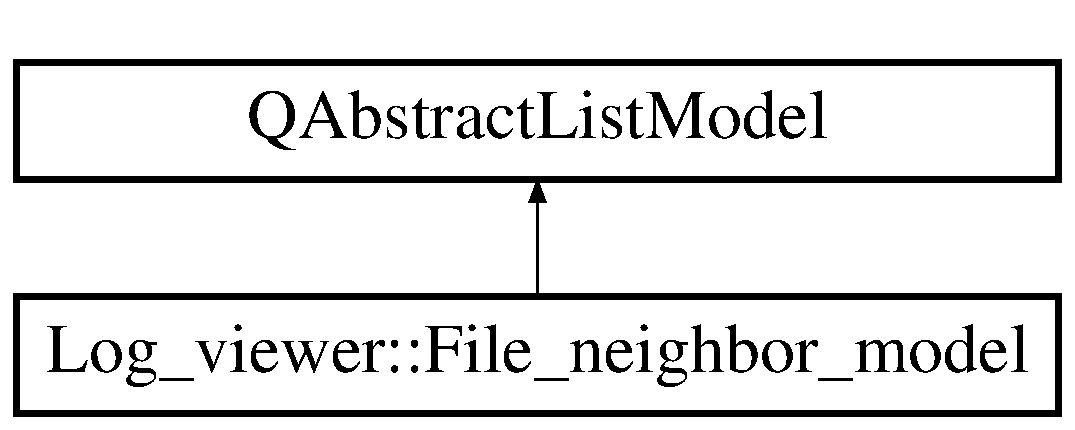
\includegraphics[height=2.000000cm]{class_log__viewer_1_1_file__neighbor__model}
\end{center}
\end{figure}
\subsection*{Public Slots}
\begin{DoxyCompactItemize}
\item 
\hypertarget{class_log__viewer_1_1_file__neighbor__model_a46b0415310949441b08c92cf6ea57aa8}{void {\bfseries on\-\_\-neighbor\-\_\-folder\-\_\-changed} (const Q\-String \&folder)}\label{class_log__viewer_1_1_file__neighbor__model_a46b0415310949441b08c92cf6ea57aa8}

\end{DoxyCompactItemize}
\subsection*{Signals}
\begin{DoxyCompactItemize}
\item 
\hypertarget{class_log__viewer_1_1_file__neighbor__model_a1f4fe308b17a3b84fbd54ffe917beab3}{void {\bfseries populated} ()}\label{class_log__viewer_1_1_file__neighbor__model_a1f4fe308b17a3b84fbd54ffe917beab3}

\end{DoxyCompactItemize}
\subsection*{Public Member Functions}
\begin{DoxyCompactItemize}
\item 
\hypertarget{class_log__viewer_1_1_file__neighbor__model_a875a577f1b7c49b96b20f31b69541b66}{{\bfseries File\-\_\-neighbor\-\_\-model} (Q\-Object $\ast$parent=0)}\label{class_log__viewer_1_1_file__neighbor__model_a875a577f1b7c49b96b20f31b69541b66}

\item 
\hypertarget{class_log__viewer_1_1_file__neighbor__model_a585628f128ef1c2d33856f8a368815b5}{int {\bfseries row\-Count} (const Q\-Model\-Index \&parent) const }\label{class_log__viewer_1_1_file__neighbor__model_a585628f128ef1c2d33856f8a368815b5}

\item 
\hypertarget{class_log__viewer_1_1_file__neighbor__model_a8f944a0893f1266cb44ceec27ede7057}{Q\-Variant {\bfseries data} (const Q\-Model\-Index \&index, int role) const }\label{class_log__viewer_1_1_file__neighbor__model_a8f944a0893f1266cb44ceec27ede7057}

\item 
\hypertarget{class_log__viewer_1_1_file__neighbor__model_a0748630f568df0d9d4b34074804db901}{void {\bfseries populate} (const Q\-String \&file\-\_\-name)}\label{class_log__viewer_1_1_file__neighbor__model_a0748630f568df0d9d4b34074804db901}

\item 
\hypertarget{class_log__viewer_1_1_file__neighbor__model_afe5a8cfeac88cc3b048cd096fdccdbe2}{void {\bfseries add} (const Q\-String \&file)}\label{class_log__viewer_1_1_file__neighbor__model_afe5a8cfeac88cc3b048cd096fdccdbe2}

\item 
\hypertarget{class_log__viewer_1_1_file__neighbor__model_a5b8f4b2a94f9d6a3b801478c8487de35}{void {\bfseries remove} (int index)}\label{class_log__viewer_1_1_file__neighbor__model_a5b8f4b2a94f9d6a3b801478c8487de35}

\item 
\hypertarget{class_log__viewer_1_1_file__neighbor__model_a6d25d14d638dfa7cc898d3384b02a354}{void {\bfseries clear} ()}\label{class_log__viewer_1_1_file__neighbor__model_a6d25d14d638dfa7cc898d3384b02a354}

\item 
\hypertarget{class_log__viewer_1_1_file__neighbor__model_aeebb698a61905772571a33be24fd9a87}{const Q\-File\-Info {\bfseries get\-\_\-item} (const Q\-Model\-Index \&index) const }\label{class_log__viewer_1_1_file__neighbor__model_aeebb698a61905772571a33be24fd9a87}

\item 
\hypertarget{class_log__viewer_1_1_file__neighbor__model_a8b72248cb145f956a107fc0b18e7b151}{void {\bfseries set\-\_\-active\-\_\-item} (int item)}\label{class_log__viewer_1_1_file__neighbor__model_a8b72248cb145f956a107fc0b18e7b151}

\item 
\hypertarget{class_log__viewer_1_1_file__neighbor__model_a4b53d2224e0b499c8751a4444b3a3bf5}{void {\bfseries set\-\_\-active\-\_\-item} (const Q\-String \&file\-\_\-name)}\label{class_log__viewer_1_1_file__neighbor__model_a4b53d2224e0b499c8751a4444b3a3bf5}

\item 
\hypertarget{class_log__viewer_1_1_file__neighbor__model_a28f8faa31549ddce1f4302dc376ce312}{int {\bfseries get\-\_\-active\-\_\-item} ()}\label{class_log__viewer_1_1_file__neighbor__model_a28f8faa31549ddce1f4302dc376ce312}

\item 
\hypertarget{class_log__viewer_1_1_file__neighbor__model_a2e4c15a713b4f29df7883725c75701a2}{void {\bfseries clear\-\_\-active\-\_\-item} ()}\label{class_log__viewer_1_1_file__neighbor__model_a2e4c15a713b4f29df7883725c75701a2}

\end{DoxyCompactItemize}


The documentation for this class was generated from the following files\-:\begin{DoxyCompactItemize}
\item 
file\-\_\-neighbor\-\_\-model.\-h\item 
file\-\_\-neighbor\-\_\-model.\-cpp\end{DoxyCompactItemize}

\hypertarget{class_log__viewer_1_1ftp__files__model}{\section{Log\-\_\-viewer\-:\-:ftp\-\_\-files\-\_\-model Class Reference}
\label{class_log__viewer_1_1ftp__files__model}\index{Log\-\_\-viewer\-::ftp\-\_\-files\-\_\-model@{Log\-\_\-viewer\-::ftp\-\_\-files\-\_\-model}}
}
Inheritance diagram for Log\-\_\-viewer\-:\-:ftp\-\_\-files\-\_\-model\-:\begin{figure}[H]
\begin{center}
\leavevmode
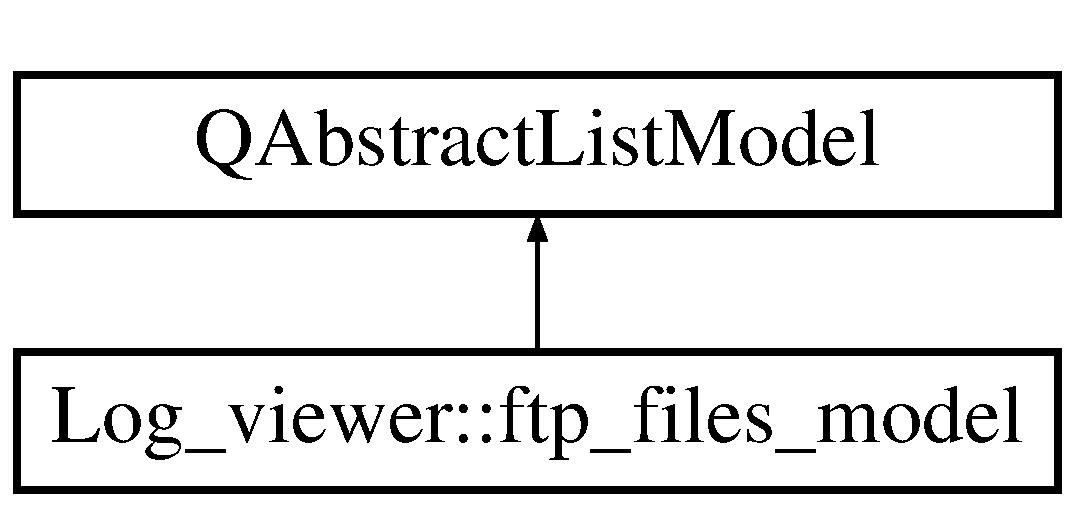
\includegraphics[height=2.000000cm]{class_log__viewer_1_1ftp__files__model}
\end{center}
\end{figure}
\subsection*{Signals}
\begin{DoxyCompactItemize}
\item 
\hypertarget{class_log__viewer_1_1ftp__files__model_a2d9ff3e9fa30a615e48a3bf4815c69b8}{void {\bfseries file\-Downloaded} (const Q\-String \&file\-Name)}\label{class_log__viewer_1_1ftp__files__model_a2d9ff3e9fa30a615e48a3bf4815c69b8}

\item 
\hypertarget{class_log__viewer_1_1ftp__files__model_ad2f6d4807002405e2fffa8d1c0df0b65}{void {\bfseries file\-Download\-Progress} (qint64 read\-Bytes, qint64 total\-Bytes)}\label{class_log__viewer_1_1ftp__files__model_ad2f6d4807002405e2fffa8d1c0df0b65}

\item 
\hypertarget{class_log__viewer_1_1ftp__files__model_a6bec2dccd8e64543972f5cb06aee8cc9}{void {\bfseries ftp\-Status\-Message} (const Q\-String \&message)}\label{class_log__viewer_1_1ftp__files__model_a6bec2dccd8e64543972f5cb06aee8cc9}

\item 
\hypertarget{class_log__viewer_1_1ftp__files__model_a305a775640096aed359d0779d00fc6c7}{void {\bfseries ftp\-Error\-Message} (const Q\-String \&message)}\label{class_log__viewer_1_1ftp__files__model_a305a775640096aed359d0779d00fc6c7}

\item 
\hypertarget{class_log__viewer_1_1ftp__files__model_aa2f7d50cab8d77944ab0810534694f57}{void {\bfseries ftp\-Connected} ()}\label{class_log__viewer_1_1ftp__files__model_aa2f7d50cab8d77944ab0810534694f57}

\item 
\hypertarget{class_log__viewer_1_1ftp__files__model_a11f002e9299bd7041f04b4436bcc3881}{void {\bfseries ftp\-Disconnected} ()}\label{class_log__viewer_1_1ftp__files__model_a11f002e9299bd7041f04b4436bcc3881}

\item 
\hypertarget{class_log__viewer_1_1ftp__files__model_a43a577bf496daf71ba7ddf8cf1547033}{void {\bfseries download\-Canceled} ()}\label{class_log__viewer_1_1ftp__files__model_a43a577bf496daf71ba7ddf8cf1547033}

\end{DoxyCompactItemize}
\subsection*{Public Member Functions}
\begin{DoxyCompactItemize}
\item 
\hypertarget{class_log__viewer_1_1ftp__files__model_a43ae08c73a9a00f51be2977c5656be77}{{\bfseries ftp\-\_\-files\-\_\-model} (Q\-Object $\ast$parent=0)}\label{class_log__viewer_1_1ftp__files__model_a43ae08c73a9a00f51be2977c5656be77}

\item 
\hypertarget{class_log__viewer_1_1ftp__files__model_a92d708869e13ae95be2ff006b40637ec}{int {\bfseries row\-Count} (const Q\-Model\-Index \&parent) const }\label{class_log__viewer_1_1ftp__files__model_a92d708869e13ae95be2ff006b40637ec}

\item 
\hypertarget{class_log__viewer_1_1ftp__files__model_a2b35513db657189098c24c1aa3d79c96}{Q\-Variant {\bfseries data} (const Q\-Model\-Index \&index, int role) const }\label{class_log__viewer_1_1ftp__files__model_a2b35513db657189098c24c1aa3d79c96}

\item 
\hypertarget{class_log__viewer_1_1ftp__files__model_aae85aeaf7540ce6c5538fd1d5728c312}{void {\bfseries connect\-To\-F\-T\-P} (const Q\-String \&host, int port, const Q\-String \&user\-Name, const Q\-String \&password)}\label{class_log__viewer_1_1ftp__files__model_aae85aeaf7540ce6c5538fd1d5728c312}

\item 
\hypertarget{class_log__viewer_1_1ftp__files__model_ae7bf3e3d84d7cafdfb321004cc2735e9}{void {\bfseries open\-File\-From\-Model\-Index} (const Q\-Model\-Index index)}\label{class_log__viewer_1_1ftp__files__model_ae7bf3e3d84d7cafdfb321004cc2735e9}

\item 
\hypertarget{class_log__viewer_1_1ftp__files__model_a6c9fd3a9e4b9eabefa67718efe838dac}{Q\-String {\bfseries format\-\_\-file\-\_\-size} (const qint64 file\-\_\-size) const }\label{class_log__viewer_1_1ftp__files__model_a6c9fd3a9e4b9eabefa67718efe838dac}

\item 
\hypertarget{class_log__viewer_1_1ftp__files__model_a2112976ac1326f47c70d3e2c88e5e158}{void {\bfseries cancel\-Download} ()}\label{class_log__viewer_1_1ftp__files__model_a2112976ac1326f47c70d3e2c88e5e158}

\end{DoxyCompactItemize}


The documentation for this class was generated from the following files\-:\begin{DoxyCompactItemize}
\item 
ftp\-\_\-files\-\_\-model.\-h\item 
ftp\-\_\-files\-\_\-model.\-cpp\end{DoxyCompactItemize}

\hypertarget{class_log__viewer_1_1_g3__log__format}{\section{Log\-\_\-viewer\-:\-:G3\-\_\-log\-\_\-format Class Reference}
\label{class_log__viewer_1_1_g3__log__format}\index{Log\-\_\-viewer\-::\-G3\-\_\-log\-\_\-format@{Log\-\_\-viewer\-::\-G3\-\_\-log\-\_\-format}}
}
Inheritance diagram for Log\-\_\-viewer\-:\-:G3\-\_\-log\-\_\-format\-:\begin{figure}[H]
\begin{center}
\leavevmode
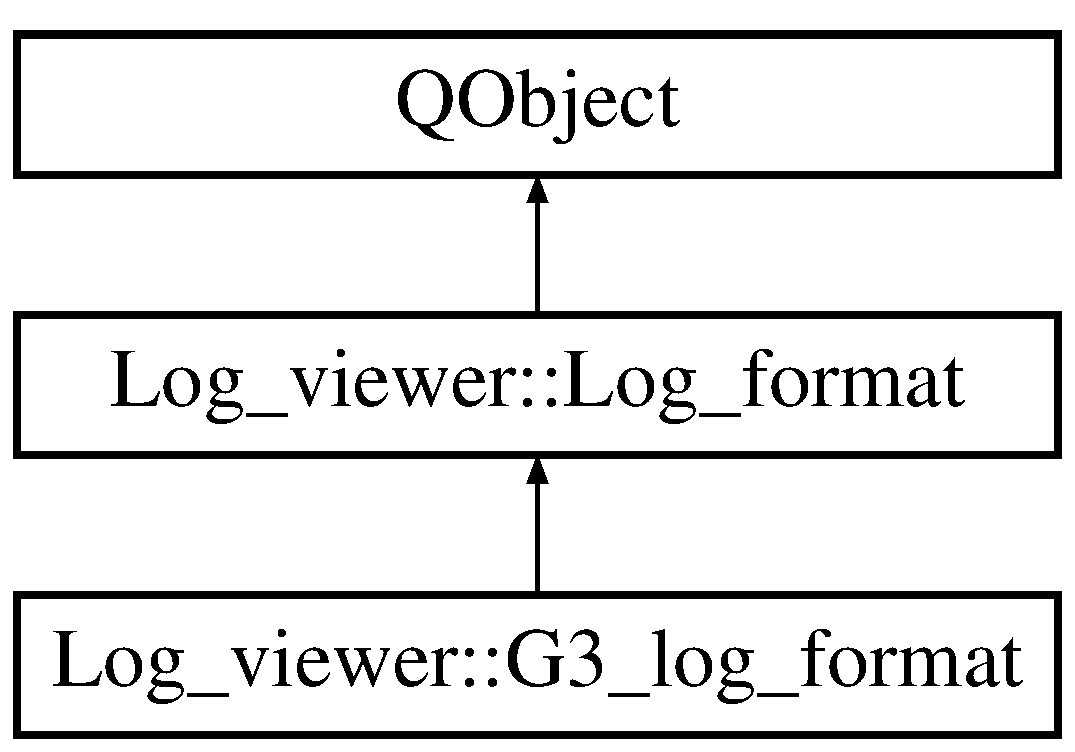
\includegraphics[height=3.000000cm]{class_log__viewer_1_1_g3__log__format}
\end{center}
\end{figure}
\subsection*{Public Member Functions}
\begin{DoxyCompactItemize}
\item 
\hypertarget{class_log__viewer_1_1_g3__log__format_aeb028cfa8a2cbe33e3af8c4a6e86baf1}{{\bfseries G3\-\_\-log\-\_\-format} (const Q\-String origin, Q\-Object $\ast$parent=0)}\label{class_log__viewer_1_1_g3__log__format_aeb028cfa8a2cbe33e3af8c4a6e86baf1}

\item 
\hypertarget{class_log__viewer_1_1_g3__log__format_a52e7429932030e6f0c3a4082c4eec18d}{bool {\bfseries match} (const Q\-String first\-\_\-line) const }\label{class_log__viewer_1_1_g3__log__format_a52e7429932030e6f0c3a4082c4eec18d}

\item 
\hypertarget{class_log__viewer_1_1_g3__log__format_a1919f49ca029f72d556d4deb8ca9432a}{Q\-String {\bfseries get\-\_\-start\-\_\-seq} () const }\label{class_log__viewer_1_1_g3__log__format_a1919f49ca029f72d556d4deb8ca9432a}

\item 
\hypertarget{class_log__viewer_1_1_g3__log__format_a1f7b4b3a5242176cc725f0a7fa611440}{Q\-String {\bfseries get\-\_\-stop\-\_\-seq} () const }\label{class_log__viewer_1_1_g3__log__format_a1f7b4b3a5242176cc725f0a7fa611440}

\item 
\hypertarget{class_log__viewer_1_1_g3__log__format_a47b38b470831ab271b03b97687e07a04}{Q\-String {\bfseries get\-\_\-description} () const }\label{class_log__viewer_1_1_g3__log__format_a47b38b470831ab271b03b97687e07a04}

\item 
\hypertarget{class_log__viewer_1_1_g3__log__format_a7a066e1f01a24945efbf5d489cd21ac3}{Q\-String {\bfseries get\-\_\-origin} () const }\label{class_log__viewer_1_1_g3__log__format_a7a066e1f01a24945efbf5d489cd21ac3}

\item 
\hypertarget{class_log__viewer_1_1_g3__log__format_a9d9748792b18f837101811d1998013d5}{Log\-\_\-columns {\bfseries get\-\_\-columns} () const }\label{class_log__viewer_1_1_g3__log__format_a9d9748792b18f837101811d1998013d5}

\end{DoxyCompactItemize}
\subsection*{Additional Inherited Members}


The documentation for this class was generated from the following file\-:\begin{DoxyCompactItemize}
\item 
g3\-\_\-log\-\_\-format.\-h\end{DoxyCompactItemize}

\hypertarget{class_log__viewer_1_1_g3__log__item}{\section{Log\-\_\-viewer\-:\-:G3\-\_\-log\-\_\-item Class Reference}
\label{class_log__viewer_1_1_g3__log__item}\index{Log\-\_\-viewer\-::\-G3\-\_\-log\-\_\-item@{Log\-\_\-viewer\-::\-G3\-\_\-log\-\_\-item}}
}
Inheritance diagram for Log\-\_\-viewer\-:\-:G3\-\_\-log\-\_\-item\-:\begin{figure}[H]
\begin{center}
\leavevmode
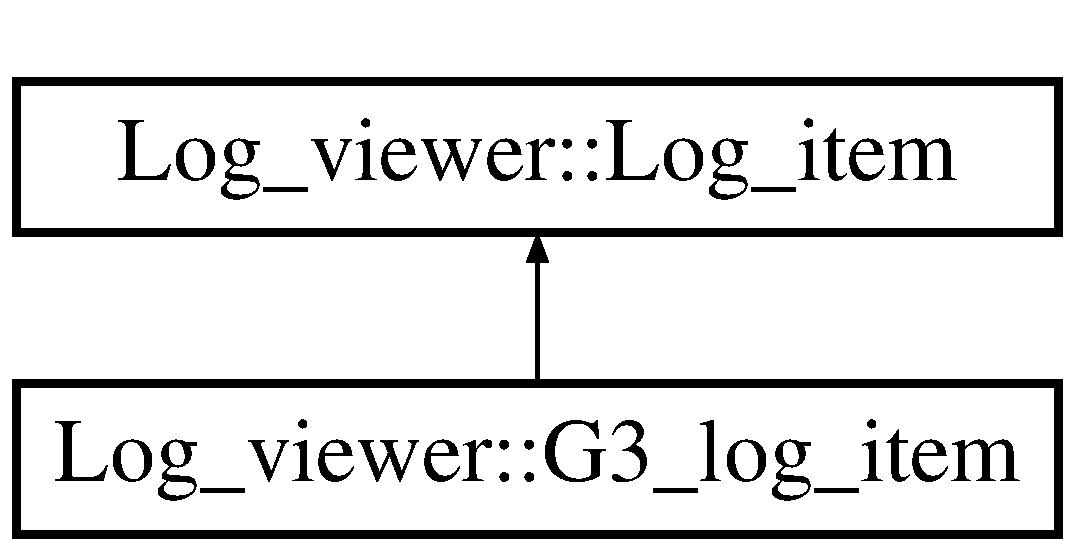
\includegraphics[height=2.000000cm]{class_log__viewer_1_1_g3__log__item}
\end{center}
\end{figure}
\subsection*{Public Member Functions}
\begin{DoxyCompactItemize}
\item 
\hypertarget{class_log__viewer_1_1_g3__log__item_a34273418bea558fe09c562f6281c9fa8}{{\bfseries G3\-\_\-log\-\_\-item} (const Q\-String value, const Q\-String separator, const Q\-String origin)}\label{class_log__viewer_1_1_g3__log__item_a34273418bea558fe09c562f6281c9fa8}

\end{DoxyCompactItemize}
\subsection*{Protected Member Functions}
\begin{DoxyCompactItemize}
\item 
\hypertarget{class_log__viewer_1_1_g3__log__item_a9c65db50792d1b5100de75f8ca72d3cf}{Log\-\_\-type {\bfseries Log\-\_\-type\-\_\-from\-\_\-string} (const Q\-String value)}\label{class_log__viewer_1_1_g3__log__item_a9c65db50792d1b5100de75f8ca72d3cf}

\end{DoxyCompactItemize}
\subsection*{Additional Inherited Members}


The documentation for this class was generated from the following files\-:\begin{DoxyCompactItemize}
\item 
g3\-\_\-log\-\_\-item.\-h\item 
g3\-\_\-log\-\_\-item.\-cpp\end{DoxyCompactItemize}

\hypertarget{class_log__viewer_1_1_log__client}{\section{Log\-\_\-viewer\-:\-:Log\-\_\-client Class Reference}
\label{class_log__viewer_1_1_log__client}\index{Log\-\_\-viewer\-::\-Log\-\_\-client@{Log\-\_\-viewer\-::\-Log\-\_\-client}}
}
Inheritance diagram for Log\-\_\-viewer\-:\-:Log\-\_\-client\-:\begin{figure}[H]
\begin{center}
\leavevmode
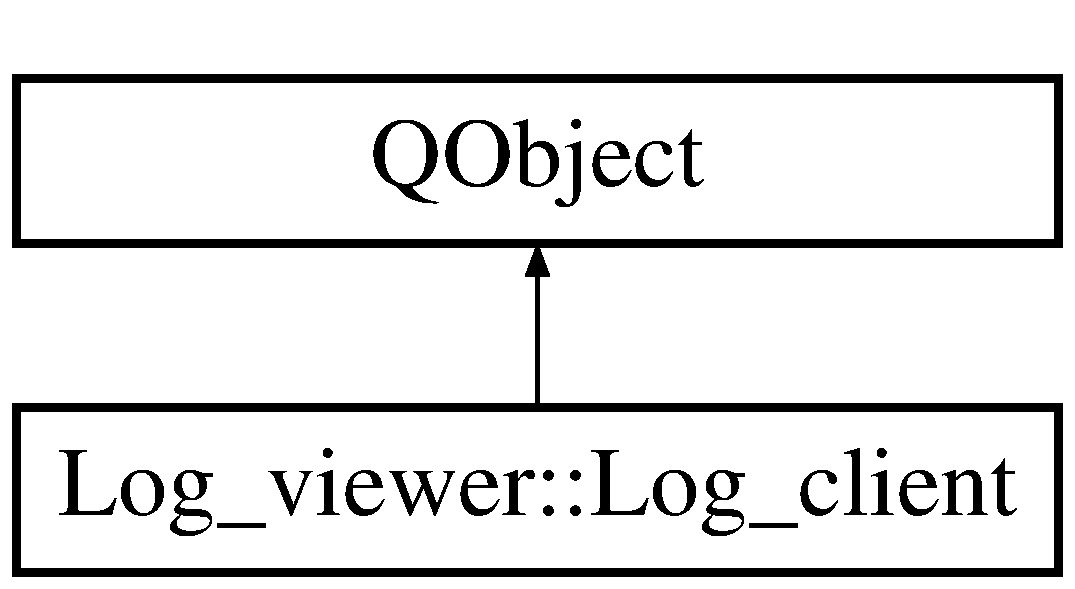
\includegraphics[height=2.000000cm]{class_log__viewer_1_1_log__client}
\end{center}
\end{figure}
\subsection*{Signals}
\begin{DoxyCompactItemize}
\item 
\hypertarget{class_log__viewer_1_1_log__client_aa33a44112924a8e930efd38a8e179bee}{void {\bfseries disconnected} (const \hyperlink{class_log__viewer_1_1_log__client}{Log\-\_\-client} $\ast$client)}\label{class_log__viewer_1_1_log__client_aa33a44112924a8e930efd38a8e179bee}

\item 
\hypertarget{class_log__viewer_1_1_log__client_a3888e37d99d0867e052e0bf199f2ad31}{void {\bfseries log\-\_\-found} (Q\-Shared\-Pointer$<$ \hyperlink{class_log__viewer_1_1_log__item}{Log\-\_\-item} $>$ log\-\_\-item)}\label{class_log__viewer_1_1_log__client_a3888e37d99d0867e052e0bf199f2ad31}

\item 
\hypertarget{class_log__viewer_1_1_log__client_af9e847fe495aaedca2dd12c9b6dc140e}{void {\bfseries format\-\_\-selected} (Q\-Shared\-Pointer$<$ \hyperlink{class_log__viewer_1_1_log__format}{Log\-\_\-format} $>$ format)}\label{class_log__viewer_1_1_log__client_af9e847fe495aaedca2dd12c9b6dc140e}

\end{DoxyCompactItemize}
\subsection*{Public Member Functions}
\begin{DoxyCompactItemize}
\item 
\hypertarget{class_log__viewer_1_1_log__client_a9acd4a9779abbe1e8d7c901957d25e08}{{\bfseries Log\-\_\-client} (Q\-Object $\ast$parent, Q\-Tcp\-Socket $\ast$socket)}\label{class_log__viewer_1_1_log__client_a9acd4a9779abbe1e8d7c901957d25e08}

\item 
\hypertarget{class_log__viewer_1_1_log__client_a4c6e877bda0d4797c4a8f828f4aba7e2}{Q\-String {\bfseries get\-\_\-address} () const }\label{class_log__viewer_1_1_log__client_a4c6e877bda0d4797c4a8f828f4aba7e2}

\end{DoxyCompactItemize}


The documentation for this class was generated from the following files\-:\begin{DoxyCompactItemize}
\item 
log\-\_\-client.\-h\item 
log\-\_\-client.\-cpp\end{DoxyCompactItemize}

\hypertarget{struct_log__viewer_1_1_log__column}{\section{Log\-\_\-viewer\-:\-:Log\-\_\-column Struct Reference}
\label{struct_log__viewer_1_1_log__column}\index{Log\-\_\-viewer\-::\-Log\-\_\-column@{Log\-\_\-viewer\-::\-Log\-\_\-column}}
}
\subsection*{Public Member Functions}
\begin{DoxyCompactItemize}
\item 
\hypertarget{struct_log__viewer_1_1_log__column_a6db03fdeca6b91116292afb7247a8a81}{{\bfseries Log\-\_\-column} (Column\-\_\-type a\-\_\-type)}\label{struct_log__viewer_1_1_log__column_a6db03fdeca6b91116292afb7247a8a81}

\item 
\hypertarget{struct_log__viewer_1_1_log__column_a19ad3f181daecd0bc4769a93558d7cfc}{Q\-String {\bfseries get\-\_\-value\-\_\-for\-\_\-log\-\_\-item} (const \hyperlink{class_log__viewer_1_1_log__item}{Log\-\_\-item} \&log\-\_\-item) const }\label{struct_log__viewer_1_1_log__column_a19ad3f181daecd0bc4769a93558d7cfc}

\end{DoxyCompactItemize}
\subsection*{Public Attributes}
\begin{DoxyCompactItemize}
\item 
\hypertarget{struct_log__viewer_1_1_log__column_ab597497e9e74bfc6fb831b2ad8464411}{Q\-String {\bfseries caption}}\label{struct_log__viewer_1_1_log__column_ab597497e9e74bfc6fb831b2ad8464411}

\item 
\hypertarget{struct_log__viewer_1_1_log__column_a77442e95e6e2e2aa8d00da1472d18bd4}{Column\-\_\-type {\bfseries type}}\label{struct_log__viewer_1_1_log__column_a77442e95e6e2e2aa8d00da1472d18bd4}

\item 
\hypertarget{struct_log__viewer_1_1_log__column_a234e917aa4e678a64db56c0621f57e97}{Q\-Size {\bfseries size\-\_\-hint}}\label{struct_log__viewer_1_1_log__column_a234e917aa4e678a64db56c0621f57e97}

\end{DoxyCompactItemize}


The documentation for this struct was generated from the following files\-:\begin{DoxyCompactItemize}
\item 
log\-\_\-column.\-h\item 
log\-\_\-column.\-cpp\end{DoxyCompactItemize}

\hypertarget{class_log__viewer_1_1_log__file__parser}{\section{Log\-\_\-viewer\-:\-:Log\-\_\-file\-\_\-parser Class Reference}
\label{class_log__viewer_1_1_log__file__parser}\index{Log\-\_\-viewer\-::\-Log\-\_\-file\-\_\-parser@{Log\-\_\-viewer\-::\-Log\-\_\-file\-\_\-parser}}
}
Inheritance diagram for Log\-\_\-viewer\-:\-:Log\-\_\-file\-\_\-parser\-:\begin{figure}[H]
\begin{center}
\leavevmode
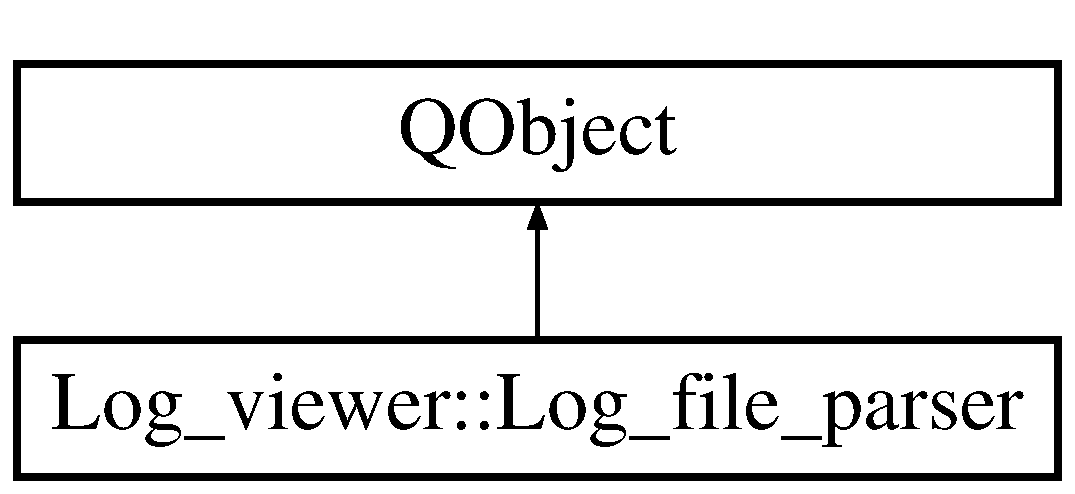
\includegraphics[height=2.000000cm]{class_log__viewer_1_1_log__file__parser}
\end{center}
\end{figure}
\subsection*{Public Types}
\begin{DoxyCompactItemize}
\item 
\hypertarget{class_log__viewer_1_1_log__file__parser_a97c54e090e5be114c70bd78661891ec4}{typedef Q\-List$<$ Q\-Shared\-Pointer\\*
$<$ \hyperlink{class_log__viewer_1_1_log__item}{Log\-\_\-item} $>$ $>$ {\bfseries Log\-\_\-items}}\label{class_log__viewer_1_1_log__file__parser_a97c54e090e5be114c70bd78661891ec4}

\end{DoxyCompactItemize}
\subsection*{Signals}
\begin{DoxyCompactItemize}
\item 
\hypertarget{class_log__viewer_1_1_log__file__parser_ab2e25ba91cab3a35612817b4afdd1daa}{void {\bfseries logs\-\_\-found} (const Log\-\_\-file\-\_\-parser\-::\-Log\-\_\-items \&log\-\_\-items)}\label{class_log__viewer_1_1_log__file__parser_ab2e25ba91cab3a35612817b4afdd1daa}

\item 
\hypertarget{class_log__viewer_1_1_log__file__parser_aa09259045d1eb36b6161c6df42ffa989}{void {\bfseries format\-\_\-selected} (Q\-Shared\-Pointer$<$ \hyperlink{class_log__viewer_1_1_log__format}{Log\-\_\-format} $>$ format)}\label{class_log__viewer_1_1_log__file__parser_aa09259045d1eb36b6161c6df42ffa989}

\item 
\hypertarget{class_log__viewer_1_1_log__file__parser_af6886ef73843c30cb49f89793109683e}{void {\bfseries file\-\_\-opened} (const Q\-String file, qint64 size)}\label{class_log__viewer_1_1_log__file__parser_af6886ef73843c30cb49f89793109683e}

\item 
\hypertarget{class_log__viewer_1_1_log__file__parser_a01c91220b455b1a5f1d123f4cdc1e904}{void {\bfseries error} (const Q\-String error)}\label{class_log__viewer_1_1_log__file__parser_a01c91220b455b1a5f1d123f4cdc1e904}

\item 
\hypertarget{class_log__viewer_1_1_log__file__parser_ab96a31ad1e9cd88b13fddbf8e27df5e5}{void {\bfseries file\-\_\-open\-\_\-progress} (int progress)}\label{class_log__viewer_1_1_log__file__parser_ab96a31ad1e9cd88b13fddbf8e27df5e5}

\end{DoxyCompactItemize}
\subsection*{Public Member Functions}
\begin{DoxyCompactItemize}
\item 
\hypertarget{class_log__viewer_1_1_log__file__parser_a308032ef6565bf34dac8c41f60704270}{{\bfseries Log\-\_\-file\-\_\-parser} (Q\-Object $\ast$parent=0)}\label{class_log__viewer_1_1_log__file__parser_a308032ef6565bf34dac8c41f60704270}

\item 
\hypertarget{class_log__viewer_1_1_log__file__parser_aa34205a80d670a8dbbec318da6b75a1a}{void {\bfseries open} (const Q\-String file)}\label{class_log__viewer_1_1_log__file__parser_aa34205a80d670a8dbbec318da6b75a1a}

\item 
\hypertarget{class_log__viewer_1_1_log__file__parser_a8ff908e5172c3d35830c3f333d928f39}{void {\bfseries open\-\_\-text} (Q\-Text\-Stream \&text\-\_\-stream)}\label{class_log__viewer_1_1_log__file__parser_a8ff908e5172c3d35830c3f333d928f39}

\item 
\hypertarget{class_log__viewer_1_1_log__file__parser_aec993a0ddf1d9d37e1398e68e1286b47}{void {\bfseries cancel} ()}\label{class_log__viewer_1_1_log__file__parser_aec993a0ddf1d9d37e1398e68e1286b47}

\item 
\hypertarget{class_log__viewer_1_1_log__file__parser_a72ed205ac6bda87dfe47c8b86bfca045}{Q\-Shared\-Pointer$<$ \hyperlink{class_log__viewer_1_1_log__format}{Log\-\_\-format} $>$ {\bfseries get\-\_\-current\-\_\-log\-\_\-format} ()}\label{class_log__viewer_1_1_log__file__parser_a72ed205ac6bda87dfe47c8b86bfca045}

\end{DoxyCompactItemize}


The documentation for this class was generated from the following files\-:\begin{DoxyCompactItemize}
\item 
log\-\_\-file\-\_\-parser.\-h\item 
log\-\_\-file\-\_\-parser.\-cpp\end{DoxyCompactItemize}

\hypertarget{class_log__viewer_1_1_log__filter__proxy__model}{\section{Log\-\_\-viewer\-:\-:Log\-\_\-filter\-\_\-proxy\-\_\-model Class Reference}
\label{class_log__viewer_1_1_log__filter__proxy__model}\index{Log\-\_\-viewer\-::\-Log\-\_\-filter\-\_\-proxy\-\_\-model@{Log\-\_\-viewer\-::\-Log\-\_\-filter\-\_\-proxy\-\_\-model}}
}
Inheritance diagram for Log\-\_\-viewer\-:\-:Log\-\_\-filter\-\_\-proxy\-\_\-model\-:\begin{figure}[H]
\begin{center}
\leavevmode
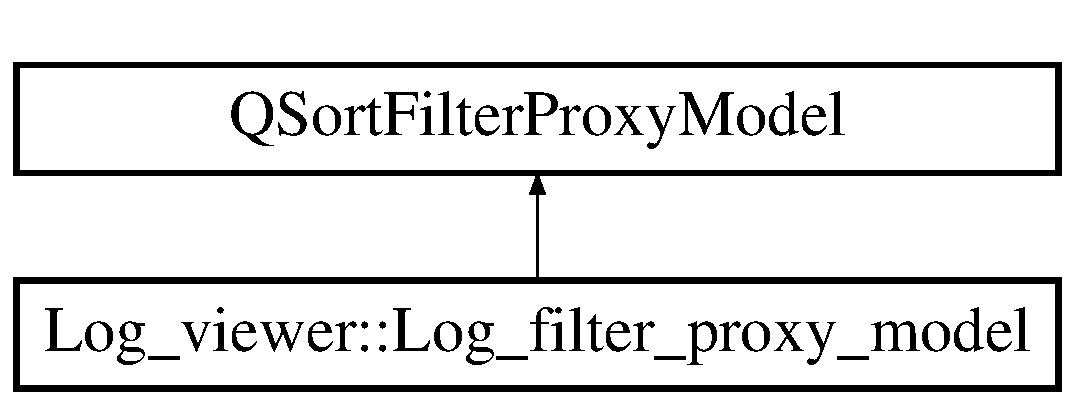
\includegraphics[height=2.000000cm]{class_log__viewer_1_1_log__filter__proxy__model}
\end{center}
\end{figure}
\subsection*{Signals}
\begin{DoxyCompactItemize}
\item 
\hypertarget{class_log__viewer_1_1_log__filter__proxy__model_af2a3a3c7f11d3c54143bb7fc45d899de}{void {\bfseries filter\-\_\-cleared} ()}\label{class_log__viewer_1_1_log__filter__proxy__model_af2a3a3c7f11d3c54143bb7fc45d899de}

\end{DoxyCompactItemize}
\subsection*{Public Member Functions}
\begin{DoxyCompactItemize}
\item 
\hypertarget{class_log__viewer_1_1_log__filter__proxy__model_a8a0d26dd0fcfe6d44f7967cffd1f1a27}{{\bfseries Log\-\_\-filter\-\_\-proxy\-\_\-model} (Q\-Object $\ast$parent=0)}\label{class_log__viewer_1_1_log__filter__proxy__model_a8a0d26dd0fcfe6d44f7967cffd1f1a27}

\item 
\hypertarget{class_log__viewer_1_1_log__filter__proxy__model_ad6caf5597814e04894c1fe9f37c3c51f}{bool {\bfseries filter\-Accepts\-Row} (int source\-\_\-row, const Q\-Model\-Index \&source\-\_\-parent) const }\label{class_log__viewer_1_1_log__filter__proxy__model_ad6caf5597814e04894c1fe9f37c3c51f}

\item 
\hypertarget{class_log__viewer_1_1_log__filter__proxy__model_a82878c711e39666f7dbf359a471c5f73}{void {\bfseries set\-\_\-text\-\_\-filter} (const Q\-String \&text)}\label{class_log__viewer_1_1_log__filter__proxy__model_a82878c711e39666f7dbf359a471c5f73}

\item 
\hypertarget{class_log__viewer_1_1_log__filter__proxy__model_aa80925a3c0856ea81c1c6dc942c896c2}{void {\bfseries set\-\_\-index\-\_\-filter} (const Q\-String \&index)}\label{class_log__viewer_1_1_log__filter__proxy__model_aa80925a3c0856ea81c1c6dc942c896c2}

\item 
\hypertarget{class_log__viewer_1_1_log__filter__proxy__model_a5dd3f3cb9936f9b32bb2baeaf7e7b9c9}{void {\bfseries set\-\_\-module\-\_\-filter} (const Q\-String \&module)}\label{class_log__viewer_1_1_log__filter__proxy__model_a5dd3f3cb9936f9b32bb2baeaf7e7b9c9}

\item 
\hypertarget{class_log__viewer_1_1_log__filter__proxy__model_a9a11f16aa4f3f4b186a365e9fb1310dd}{void {\bfseries set\-\_\-file\-\_\-filter} (const Q\-String \&file)}\label{class_log__viewer_1_1_log__filter__proxy__model_a9a11f16aa4f3f4b186a365e9fb1310dd}

\item 
\hypertarget{class_log__viewer_1_1_log__filter__proxy__model_a490ed1c25beba6aebc0e300d9425e100}{void {\bfseries add\-\_\-type\-\_\-filter} (Log\-\_\-type type)}\label{class_log__viewer_1_1_log__filter__proxy__model_a490ed1c25beba6aebc0e300d9425e100}

\item 
\hypertarget{class_log__viewer_1_1_log__filter__proxy__model_ad56a9dcdb23173dbe40fbdd68c7a03b5}{void {\bfseries clear\-\_\-type\-\_\-filter} ()}\label{class_log__viewer_1_1_log__filter__proxy__model_ad56a9dcdb23173dbe40fbdd68c7a03b5}

\item 
\hypertarget{class_log__viewer_1_1_log__filter__proxy__model_adb482b98080b7ed6f9aa1f34b3a2be7f}{void {\bfseries clear\-\_\-filter} ()}\label{class_log__viewer_1_1_log__filter__proxy__model_adb482b98080b7ed6f9aa1f34b3a2be7f}

\item 
\hypertarget{class_log__viewer_1_1_log__filter__proxy__model_a14b4dfcceb4292d59633db8ba0b4281a}{void {\bfseries apply} ()}\label{class_log__viewer_1_1_log__filter__proxy__model_a14b4dfcceb4292d59633db8ba0b4281a}

\item 
\hypertarget{class_log__viewer_1_1_log__filter__proxy__model_a2ecf8154a48bef95af5048d06044c44a}{void {\bfseries set\-\_\-use\-\_\-regex} (bool enabled)}\label{class_log__viewer_1_1_log__filter__proxy__model_a2ecf8154a48bef95af5048d06044c44a}

\item 
\hypertarget{class_log__viewer_1_1_log__filter__proxy__model_a85b64917da78419d9ddef15feab2ed2e}{Q\-String {\bfseries get\-\_\-text\-\_\-filter} ()}\label{class_log__viewer_1_1_log__filter__proxy__model_a85b64917da78419d9ddef15feab2ed2e}

\end{DoxyCompactItemize}


The documentation for this class was generated from the following files\-:\begin{DoxyCompactItemize}
\item 
log\-\_\-filter\-\_\-proxy\-\_\-model.\-h\item 
log\-\_\-filter\-\_\-proxy\-\_\-model.\-cpp\end{DoxyCompactItemize}

\hypertarget{class_log__viewer_1_1_log__format}{\section{Log\-\_\-viewer\-:\-:Log\-\_\-format Class Reference}
\label{class_log__viewer_1_1_log__format}\index{Log\-\_\-viewer\-::\-Log\-\_\-format@{Log\-\_\-viewer\-::\-Log\-\_\-format}}
}
Inheritance diagram for Log\-\_\-viewer\-:\-:Log\-\_\-format\-:\begin{figure}[H]
\begin{center}
\leavevmode
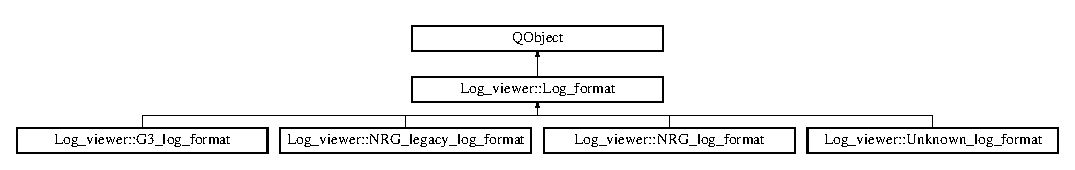
\includegraphics[height=1.834061cm]{class_log__viewer_1_1_log__format}
\end{center}
\end{figure}
\subsection*{Public Slots}
\begin{DoxyCompactItemize}
\item 
\hypertarget{class_log__viewer_1_1_log__format_a8f78b9e76b3dda71bbb5623baf4bcceb}{void {\bfseries on\-\_\-line\-\_\-found} (const Q\-String value)}\label{class_log__viewer_1_1_log__format_a8f78b9e76b3dda71bbb5623baf4bcceb}

\end{DoxyCompactItemize}
\subsection*{Signals}
\begin{DoxyCompactItemize}
\item 
\hypertarget{class_log__viewer_1_1_log__format_a7fa71ac3f12445ddb387a53343eddd6a}{void {\bfseries log\-\_\-found} (Q\-Shared\-Pointer$<$ \hyperlink{class_log__viewer_1_1_log__item}{Log\-\_\-item} $>$ item)}\label{class_log__viewer_1_1_log__format_a7fa71ac3f12445ddb387a53343eddd6a}

\end{DoxyCompactItemize}
\subsection*{Public Member Functions}
\begin{DoxyCompactItemize}
\item 
\hypertarget{class_log__viewer_1_1_log__format_aff06d1d34615bb6dc78a9f60f0800c90}{{\bfseries Log\-\_\-format} (Q\-Object $\ast$parent=0)}\label{class_log__viewer_1_1_log__format_aff06d1d34615bb6dc78a9f60f0800c90}

\item 
\hypertarget{class_log__viewer_1_1_log__format_a3bd09d2462e25b91ebb881d59220c49f}{virtual Q\-String {\bfseries get\-\_\-description} () const =0}\label{class_log__viewer_1_1_log__format_a3bd09d2462e25b91ebb881d59220c49f}

\item 
\hypertarget{class_log__viewer_1_1_log__format_a40d9e1b2a2ab55338060b16fa3979869}{virtual Q\-String {\bfseries get\-\_\-start\-\_\-seq} () const =0}\label{class_log__viewer_1_1_log__format_a40d9e1b2a2ab55338060b16fa3979869}

\item 
\hypertarget{class_log__viewer_1_1_log__format_a5f446a4324a53f918d726a727196d68b}{virtual Q\-String {\bfseries get\-\_\-stop\-\_\-seq} () const =0}\label{class_log__viewer_1_1_log__format_a5f446a4324a53f918d726a727196d68b}

\item 
\hypertarget{class_log__viewer_1_1_log__format_af939ec33a9759e25f56370fdb2a51e0b}{virtual Q\-String {\bfseries get\-\_\-origin} () const =0}\label{class_log__viewer_1_1_log__format_af939ec33a9759e25f56370fdb2a51e0b}

\item 
\hypertarget{class_log__viewer_1_1_log__format_a13dfc251301e3780f5427ed9f628a573}{virtual bool {\bfseries match} (const Q\-String first\-\_\-line) const =0}\label{class_log__viewer_1_1_log__format_a13dfc251301e3780f5427ed9f628a573}

\item 
\hypertarget{class_log__viewer_1_1_log__format_a58a93549369eb680aad0075d705c8c62}{virtual Log\-\_\-columns {\bfseries get\-\_\-columns} () const =0}\label{class_log__viewer_1_1_log__format_a58a93549369eb680aad0075d705c8c62}

\item 
\hypertarget{class_log__viewer_1_1_log__format_af2697cec3901d17a23d9107c4fd01ada}{virtual void {\bfseries add\-\_\-line} (const Q\-String line)}\label{class_log__viewer_1_1_log__format_af2697cec3901d17a23d9107c4fd01ada}

\end{DoxyCompactItemize}


The documentation for this class was generated from the following files\-:\begin{DoxyCompactItemize}
\item 
log\-\_\-format.\-h\item 
log\-\_\-format.\-cpp\end{DoxyCompactItemize}

\hypertarget{class_log__viewer_1_1_log__format__factory}{\section{Log\-\_\-viewer\-:\-:Log\-\_\-format\-\_\-factory Class Reference}
\label{class_log__viewer_1_1_log__format__factory}\index{Log\-\_\-viewer\-::\-Log\-\_\-format\-\_\-factory@{Log\-\_\-viewer\-::\-Log\-\_\-format\-\_\-factory}}
}
\subsection*{Public Member Functions}
\begin{DoxyCompactItemize}
\item 
\hypertarget{class_log__viewer_1_1_log__format__factory_a4ef6441f33c9a8b6392dcd7b082addb8}{Q\-Shared\-Pointer$<$ \hyperlink{class_log__viewer_1_1_log__format}{Log\-\_\-format} $>$ {\bfseries create} (const Q\-String first\-\_\-line, const Q\-String origin)}\label{class_log__viewer_1_1_log__format__factory_a4ef6441f33c9a8b6392dcd7b082addb8}

\end{DoxyCompactItemize}
\subsection*{Static Public Attributes}
\begin{DoxyCompactItemize}
\item 
\hypertarget{class_log__viewer_1_1_log__format__factory_a3eadcfd3d62ff681313c8e5809507ed1}{static \hyperlink{class_log__viewer_1_1_log__format__factory}{Log\-\_\-format\-\_\-factory} $\ast$ {\bfseries instance} = \&\hyperlink{class_singleton}{Singleton}$<$\hyperlink{class_log__viewer_1_1_log__format__factory}{Log\-\_\-format\-\_\-factory}$>$\-::Instance()}\label{class_log__viewer_1_1_log__format__factory_a3eadcfd3d62ff681313c8e5809507ed1}

\end{DoxyCompactItemize}


The documentation for this class was generated from the following files\-:\begin{DoxyCompactItemize}
\item 
Log\-\_\-format\-\_\-factory.\-h\item 
Log\-\_\-format\-\_\-factory.\-cpp\end{DoxyCompactItemize}

\hypertarget{class_log__viewer_1_1_log__item}{\section{Log\-\_\-viewer\-:\-:Log\-\_\-item Class Reference}
\label{class_log__viewer_1_1_log__item}\index{Log\-\_\-viewer\-::\-Log\-\_\-item@{Log\-\_\-viewer\-::\-Log\-\_\-item}}
}
Inheritance diagram for Log\-\_\-viewer\-:\-:Log\-\_\-item\-:\begin{figure}[H]
\begin{center}
\leavevmode
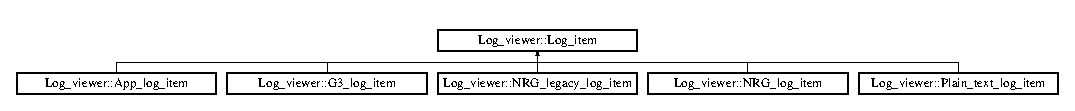
\includegraphics[height=1.037037cm]{class_log__viewer_1_1_log__item}
\end{center}
\end{figure}
\subsection*{Public Member Functions}
\begin{DoxyCompactItemize}
\item 
\hypertarget{class_log__viewer_1_1_log__item_ab518dfa8ffa70dcadfc57d65c5f452f2}{Q\-String {\bfseries get\-\_\-log\-\_\-type\-\_\-as\-\_\-string} () const }\label{class_log__viewer_1_1_log__item_ab518dfa8ffa70dcadfc57d65c5f452f2}

\item 
\hypertarget{class_log__viewer_1_1_log__item_ae680189e0ae3c28a5a3d3d5639a2718a}{Log\-\_\-type {\bfseries get\-\_\-log\-\_\-type} () const }\label{class_log__viewer_1_1_log__item_ae680189e0ae3c28a5a3d3d5639a2718a}

\item 
\hypertarget{class_log__viewer_1_1_log__item_a9311ac6bf9998010b63bbcf050895296}{Q\-String {\bfseries get\-\_\-text} () const }\label{class_log__viewer_1_1_log__item_a9311ac6bf9998010b63bbcf050895296}

\item 
\hypertarget{class_log__viewer_1_1_log__item_ad87addf407e7060b161c5e482fb296c8}{Q\-String {\bfseries get\-\_\-date} () const }\label{class_log__viewer_1_1_log__item_ad87addf407e7060b161c5e482fb296c8}

\item 
\hypertarget{class_log__viewer_1_1_log__item_abe7bf92fdc4c5efe0263d9ab6ddc7c3e}{Q\-String {\bfseries get\-\_\-time} () const }\label{class_log__viewer_1_1_log__item_abe7bf92fdc4c5efe0263d9ab6ddc7c3e}

\item 
\hypertarget{class_log__viewer_1_1_log__item_a71f518f482459697abf7f48f1d5611a7}{Q\-String {\bfseries get\-\_\-file} () const }\label{class_log__viewer_1_1_log__item_a71f518f482459697abf7f48f1d5611a7}

\item 
\hypertarget{class_log__viewer_1_1_log__item_ab18ec2426da2f6c15377eff8af273ad0}{Q\-String {\bfseries get\-\_\-method} () const }\label{class_log__viewer_1_1_log__item_ab18ec2426da2f6c15377eff8af273ad0}

\item 
\hypertarget{class_log__viewer_1_1_log__item_aa6d5182cd7135cbc010d5e2ac096b69a}{Q\-String {\bfseries get\-\_\-line} () const }\label{class_log__viewer_1_1_log__item_aa6d5182cd7135cbc010d5e2ac096b69a}

\item 
\hypertarget{class_log__viewer_1_1_log__item_a5ea07087e1c69b7b47f9e086c9dc7805}{Q\-String {\bfseries get\-\_\-application} () const }\label{class_log__viewer_1_1_log__item_a5ea07087e1c69b7b47f9e086c9dc7805}

\item 
\hypertarget{class_log__viewer_1_1_log__item_a3d66e3ad889dead96d86d071f8fbb953}{Q\-String {\bfseries get\-\_\-module} () const }\label{class_log__viewer_1_1_log__item_a3d66e3ad889dead96d86d071f8fbb953}

\item 
\hypertarget{class_log__viewer_1_1_log__item_a30e41f8ef5414fea09f3956214fdf847}{Q\-String {\bfseries get\-\_\-thread} () const }\label{class_log__viewer_1_1_log__item_a30e41f8ef5414fea09f3956214fdf847}

\item 
\hypertarget{class_log__viewer_1_1_log__item_a689335f055faa87775bff3a70c684782}{Q\-String {\bfseries get\-\_\-origin} () const }\label{class_log__viewer_1_1_log__item_a689335f055faa87775bff3a70c684782}

\item 
\hypertarget{class_log__viewer_1_1_log__item_a0e4cbe313f42e8b39089a0366211748d}{int {\bfseries get\-\_\-index} () const }\label{class_log__viewer_1_1_log__item_a0e4cbe313f42e8b39089a0366211748d}

\item 
\hypertarget{class_log__viewer_1_1_log__item_a75044accf5b403e2df600b0400f43a19}{void {\bfseries set\-\_\-index} (int index)}\label{class_log__viewer_1_1_log__item_a75044accf5b403e2df600b0400f43a19}

\item 
\hypertarget{class_log__viewer_1_1_log__item_a07cf45b193c545d618a0d31f84589edd}{Q\-String {\bfseries get\-\_\-as\-\_\-string} (const Q\-String \&separator) const }\label{class_log__viewer_1_1_log__item_a07cf45b193c545d618a0d31f84589edd}

\end{DoxyCompactItemize}
\subsection*{Static Public Member Functions}
\begin{DoxyCompactItemize}
\item 
\hypertarget{class_log__viewer_1_1_log__item_a247847a2d6a0c18666a52198e6826752}{static Q\-String {\bfseries get\-\_\-log\-\_\-type\-\_\-as\-\_\-string} (Log\-\_\-type type)}\label{class_log__viewer_1_1_log__item_a247847a2d6a0c18666a52198e6826752}

\end{DoxyCompactItemize}
\subsection*{Protected Member Functions}
\begin{DoxyCompactItemize}
\item 
\hypertarget{class_log__viewer_1_1_log__item_a97a3177b547998c85e497be12c388997}{virtual Log\-\_\-type {\bfseries Log\-\_\-type\-\_\-from\-\_\-string} (const Q\-String value)=0}\label{class_log__viewer_1_1_log__item_a97a3177b547998c85e497be12c388997}

\end{DoxyCompactItemize}
\subsection*{Protected Attributes}
\begin{DoxyCompactItemize}
\item 
\hypertarget{class_log__viewer_1_1_log__item_adde025c2219cbd05f2014d7224367af1}{int {\bfseries m\-\_\-index}}\label{class_log__viewer_1_1_log__item_adde025c2219cbd05f2014d7224367af1}

\item 
\hypertarget{class_log__viewer_1_1_log__item_ae9bfe83e483c11715490af2c512005c1}{Log\-\_\-type {\bfseries m\-\_\-type}}\label{class_log__viewer_1_1_log__item_ae9bfe83e483c11715490af2c512005c1}

\item 
\hypertarget{class_log__viewer_1_1_log__item_a05fe9e44146f48eef7dffa058f499452}{Q\-String {\bfseries m\-\_\-text}}\label{class_log__viewer_1_1_log__item_a05fe9e44146f48eef7dffa058f499452}

\item 
\hypertarget{class_log__viewer_1_1_log__item_acfdb4db1c5c6371994360fa35b47af79}{Q\-String {\bfseries m\-\_\-date}}\label{class_log__viewer_1_1_log__item_acfdb4db1c5c6371994360fa35b47af79}

\item 
\hypertarget{class_log__viewer_1_1_log__item_a58f8072adef8fa33f153cd5c6539d547}{Q\-String {\bfseries m\-\_\-time}}\label{class_log__viewer_1_1_log__item_a58f8072adef8fa33f153cd5c6539d547}

\item 
\hypertarget{class_log__viewer_1_1_log__item_a36fee5d4eb92261682670da7373bd155}{Q\-String {\bfseries m\-\_\-file}}\label{class_log__viewer_1_1_log__item_a36fee5d4eb92261682670da7373bd155}

\item 
\hypertarget{class_log__viewer_1_1_log__item_a70468fa5bfc1e5c0f055a277699bc1f0}{Q\-String {\bfseries m\-\_\-method}}\label{class_log__viewer_1_1_log__item_a70468fa5bfc1e5c0f055a277699bc1f0}

\item 
\hypertarget{class_log__viewer_1_1_log__item_ad4da52eae6438467b4711ca9505efcc4}{Q\-String {\bfseries m\-\_\-line}}\label{class_log__viewer_1_1_log__item_ad4da52eae6438467b4711ca9505efcc4}

\item 
\hypertarget{class_log__viewer_1_1_log__item_a8991da3b514bd800d8b1b03a0aa50b5b}{Q\-String {\bfseries m\-\_\-application}}\label{class_log__viewer_1_1_log__item_a8991da3b514bd800d8b1b03a0aa50b5b}

\item 
\hypertarget{class_log__viewer_1_1_log__item_adb2b8746a2b59404dfbcf77ac557e7f9}{Q\-String {\bfseries m\-\_\-module}}\label{class_log__viewer_1_1_log__item_adb2b8746a2b59404dfbcf77ac557e7f9}

\item 
\hypertarget{class_log__viewer_1_1_log__item_af97cbe89d09438bf284b5ba48f64a810}{Q\-String {\bfseries m\-\_\-thread}}\label{class_log__viewer_1_1_log__item_af97cbe89d09438bf284b5ba48f64a810}

\item 
\hypertarget{class_log__viewer_1_1_log__item_a3e27163b918b9ac0dac0ce30e2f12a0c}{Q\-String {\bfseries m\-\_\-origin}}\label{class_log__viewer_1_1_log__item_a3e27163b918b9ac0dac0ce30e2f12a0c}

\end{DoxyCompactItemize}


The documentation for this class was generated from the following files\-:\begin{DoxyCompactItemize}
\item 
log\-\_\-item.\-h\item 
log\-\_\-item.\-cpp\end{DoxyCompactItemize}

\hypertarget{class_log__item__preview__text_edit}{\section{Log\-\_\-item\-\_\-preview\-\_\-text\-Edit Class Reference}
\label{class_log__item__preview__text_edit}\index{Log\-\_\-item\-\_\-preview\-\_\-text\-Edit@{Log\-\_\-item\-\_\-preview\-\_\-text\-Edit}}
}
Inheritance diagram for Log\-\_\-item\-\_\-preview\-\_\-text\-Edit\-:\begin{figure}[H]
\begin{center}
\leavevmode
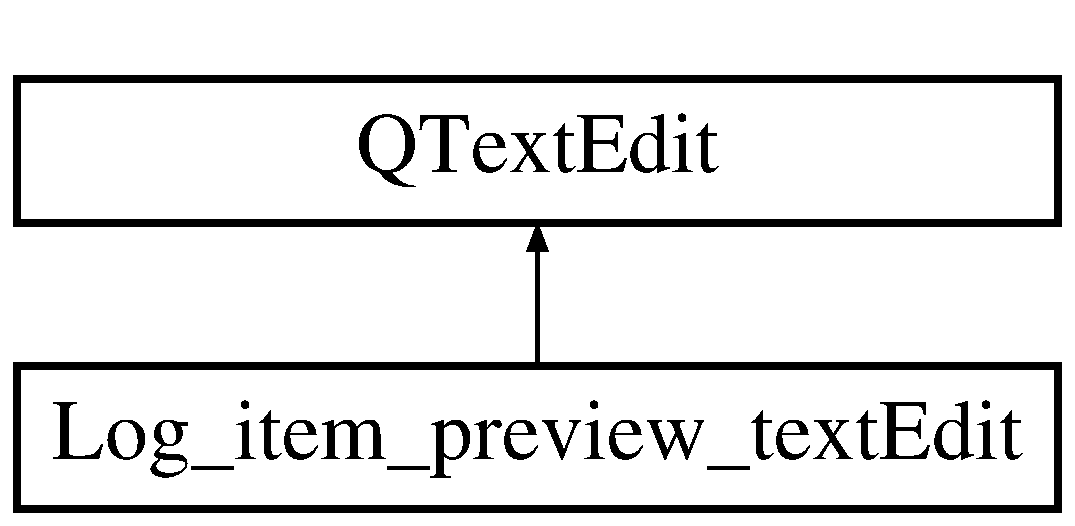
\includegraphics[height=2.000000cm]{class_log__item__preview__text_edit}
\end{center}
\end{figure}
\subsection*{Public Types}
\begin{DoxyCompactItemize}
\item 
\hypertarget{class_log__item__preview__text_edit_a21369eab2c7fe8d8dd3e3c3411f0b6e4}{typedef Q\-Pair$<$ Q\-String, Q\-Color $>$ {\bfseries String\-\_\-color\-\_\-pair}}\label{class_log__item__preview__text_edit_a21369eab2c7fe8d8dd3e3c3411f0b6e4}

\item 
\hypertarget{class_log__item__preview__text_edit_a2e558af15bd3237aadfe8c594c600c3d}{typedef Q\-List$<$ String\-\_\-color\-\_\-pair $>$ {\bfseries String\-\_\-color\-\_\-list}}\label{class_log__item__preview__text_edit_a2e558af15bd3237aadfe8c594c600c3d}

\end{DoxyCompactItemize}
\subsection*{Public Member Functions}
\begin{DoxyCompactItemize}
\item 
\hypertarget{class_log__item__preview__text_edit_ad38f39a5635662a9720661c2adc1a707}{{\bfseries Log\-\_\-item\-\_\-preview\-\_\-text\-Edit} (Q\-Widget $\ast$parent=0)}\label{class_log__item__preview__text_edit_ad38f39a5635662a9720661c2adc1a707}

\item 
\hypertarget{class_log__item__preview__text_edit_a4c6a931ec095bf471ba7a6239851e8e3}{void {\bfseries show\-\_\-item} (const Q\-String \&row, const Q\-String \&text, const Q\-String \&type, const Q\-String \&file, const Q\-String \&line, const Q\-String \&origin, const String\-\_\-color\-\_\-list \&list, const Q\-String \&filter\-\_\-text)}\label{class_log__item__preview__text_edit_a4c6a931ec095bf471ba7a6239851e8e3}

\item 
\hypertarget{class_log__item__preview__text_edit_a632986f2540bbbdf480214156b73538e}{void {\bfseries clear\-\_\-item} ()}\label{class_log__item__preview__text_edit_a632986f2540bbbdf480214156b73538e}

\end{DoxyCompactItemize}


The documentation for this class was generated from the following files\-:\begin{DoxyCompactItemize}
\item 
log\-\_\-item\-\_\-preview\-\_\-textedit.\-h\item 
log\-\_\-item\-\_\-preview\-\_\-textedit.\-cpp\end{DoxyCompactItemize}

\hypertarget{class_log__viewer_1_1_log__items__model}{\section{Log\-\_\-viewer\-:\-:Log\-\_\-items\-\_\-model Class Reference}
\label{class_log__viewer_1_1_log__items__model}\index{Log\-\_\-viewer\-::\-Log\-\_\-items\-\_\-model@{Log\-\_\-viewer\-::\-Log\-\_\-items\-\_\-model}}
}
Inheritance diagram for Log\-\_\-viewer\-:\-:Log\-\_\-items\-\_\-model\-:\begin{figure}[H]
\begin{center}
\leavevmode
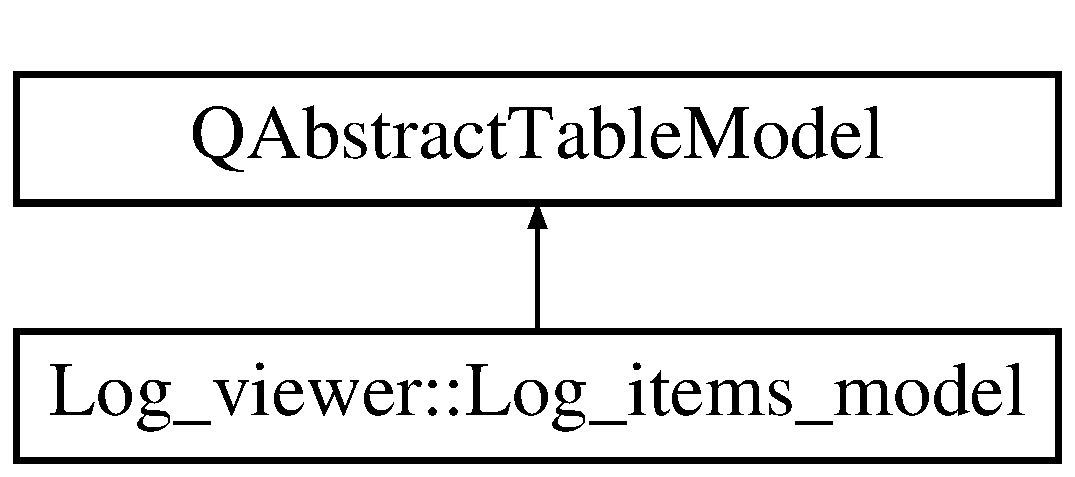
\includegraphics[height=2.000000cm]{class_log__viewer_1_1_log__items__model}
\end{center}
\end{figure}
\subsection*{Public Types}
\begin{DoxyCompactItemize}
\item 
\hypertarget{class_log__viewer_1_1_log__items__model_af4fa93fd2a023946a84a8e6cb913c11e}{typedef Q\-Pair$<$ Q\-String, Q\-Color $>$ {\bfseries Highlight\-\_\-text\-\_\-pair}}\label{class_log__viewer_1_1_log__items__model_af4fa93fd2a023946a84a8e6cb913c11e}

\item 
\hypertarget{class_log__viewer_1_1_log__items__model_a1775182799f950e0430d9431a2acc098}{typedef Q\-List\\*
$<$ Highlight\-\_\-text\-\_\-pair $>$ {\bfseries Color\-\_\-list}}\label{class_log__viewer_1_1_log__items__model_a1775182799f950e0430d9431a2acc098}

\end{DoxyCompactItemize}
\subsection*{Public Member Functions}
\begin{DoxyCompactItemize}
\item 
\hypertarget{class_log__viewer_1_1_log__items__model_ab38f8287204eee07e56f7f760d332b60}{{\bfseries Log\-\_\-items\-\_\-model} (Q\-Object $\ast$parent=0)}\label{class_log__viewer_1_1_log__items__model_ab38f8287204eee07e56f7f760d332b60}

\item 
\hypertarget{class_log__viewer_1_1_log__items__model_a36ce1d33ee6a53e762413e91606971e5}{int {\bfseries row\-Count} (const Q\-Model\-Index \&parent) const }\label{class_log__viewer_1_1_log__items__model_a36ce1d33ee6a53e762413e91606971e5}

\item 
\hypertarget{class_log__viewer_1_1_log__items__model_ad3608891e3d6add9b5ca6cbaf042f9e8}{int {\bfseries column\-Count} (const Q\-Model\-Index \&parent) const }\label{class_log__viewer_1_1_log__items__model_ad3608891e3d6add9b5ca6cbaf042f9e8}

\item 
\hypertarget{class_log__viewer_1_1_log__items__model_aa703d582b1947c4bd1ec08cb9ab14464}{Q\-Variant {\bfseries data} (const Q\-Model\-Index \&index, int role) const }\label{class_log__viewer_1_1_log__items__model_aa703d582b1947c4bd1ec08cb9ab14464}

\item 
\hypertarget{class_log__viewer_1_1_log__items__model_a5f242a7d86c3a41f49d2838492a5e8f2}{Q\-Variant {\bfseries header\-Data} (int section, Qt\-::\-Orientation orientation, int role) const }\label{class_log__viewer_1_1_log__items__model_a5f242a7d86c3a41f49d2838492a5e8f2}

\item 
\hypertarget{class_log__viewer_1_1_log__items__model_a54494daa82c96c64369cac5d5873ea7a}{void {\bfseries set\-\_\-columns} (const Log\-\_\-columns \&columns)}\label{class_log__viewer_1_1_log__items__model_a54494daa82c96c64369cac5d5873ea7a}

\item 
\hypertarget{class_log__viewer_1_1_log__items__model_a8975bf848715c81e639d2d1c3a841020}{void {\bfseries add} (Q\-Shared\-Pointer$<$ \hyperlink{class_log__viewer_1_1_log__item}{Log\-\_\-item} $>$ item)}\label{class_log__viewer_1_1_log__items__model_a8975bf848715c81e639d2d1c3a841020}

\item 
\hypertarget{class_log__viewer_1_1_log__items__model_a2065c7f09cf2f34bc476c9d549d4d8ba}{void {\bfseries add} (const Log\-\_\-file\-\_\-parser\-::\-Log\-\_\-items \&items)}\label{class_log__viewer_1_1_log__items__model_a2065c7f09cf2f34bc476c9d549d4d8ba}

\item 
\hypertarget{class_log__viewer_1_1_log__items__model_af90dd226e157a6629d669b0d381df5b3}{void {\bfseries clear} ()}\label{class_log__viewer_1_1_log__items__model_af90dd226e157a6629d669b0d381df5b3}

\item 
\hypertarget{class_log__viewer_1_1_log__items__model_a19c2785185c97acf5d2d94e7884656b2}{Q\-Shared\-Pointer$<$ \hyperlink{class_log__viewer_1_1_log__item}{Log\-\_\-item} $>$ {\bfseries get\-\_\-item\-\_\-at} (int index)}\label{class_log__viewer_1_1_log__items__model_a19c2785185c97acf5d2d94e7884656b2}

\item 
\hypertarget{class_log__viewer_1_1_log__items__model_ab94931c3cae966d04415071da272cfb7}{void {\bfseries add\-\_\-highlight} (const Q\-Color \&color, const Q\-String \&text)}\label{class_log__viewer_1_1_log__items__model_ab94931c3cae966d04415071da272cfb7}

\item 
\hypertarget{class_log__viewer_1_1_log__items__model_a5bfe5f0d114e990b1139102860162379}{void {\bfseries clear\-\_\-highlight} (const Q\-Color \&color)}\label{class_log__viewer_1_1_log__items__model_a5bfe5f0d114e990b1139102860162379}

\item 
\hypertarget{class_log__viewer_1_1_log__items__model_ab79792cd16b66ef42b644b0660c94e3e}{void {\bfseries clear\-\_\-all\-\_\-highlights} ()}\label{class_log__viewer_1_1_log__items__model_ab79792cd16b66ef42b644b0660c94e3e}

\item 
\hypertarget{class_log__viewer_1_1_log__items__model_ac4abf3f20d17ade1eec7b63b5b38ae38}{void {\bfseries begin\-\_\-highlight} ()}\label{class_log__viewer_1_1_log__items__model_ac4abf3f20d17ade1eec7b63b5b38ae38}

\item 
\hypertarget{class_log__viewer_1_1_log__items__model_a175e6ed971ea20ae342d1c53cdfed7e6}{void {\bfseries end\-\_\-highlight} ()}\label{class_log__viewer_1_1_log__items__model_a175e6ed971ea20ae342d1c53cdfed7e6}

\item 
\hypertarget{class_log__viewer_1_1_log__items__model_aec79939e6844d655e2444b4495fd4483}{const Color\-\_\-list {\bfseries get\-\_\-highlights} () const }\label{class_log__viewer_1_1_log__items__model_aec79939e6844d655e2444b4495fd4483}

\item 
\hypertarget{class_log__viewer_1_1_log__items__model_a4c70981f49821218b04e56e37044b86f}{void {\bfseries set\-\_\-type\-\_\-highlight} (bool enabled)}\label{class_log__viewer_1_1_log__items__model_a4c70981f49821218b04e56e37044b86f}

\item 
\hypertarget{class_log__viewer_1_1_log__items__model_a07d88207be51cb27ebd41c818ef4ada6}{void {\bfseries set\-\_\-use\-\_\-regex\-\_\-for\-\_\-highlight} (bool enabled)}\label{class_log__viewer_1_1_log__items__model_a07d88207be51cb27ebd41c818ef4ada6}

\item 
\hypertarget{class_log__viewer_1_1_log__items__model_aa63a8057f03e78a5f2191f953d6be5db}{bool {\bfseries get\-\_\-use\-\_\-regex\-\_\-for\-\_\-highlight} ()}\label{class_log__viewer_1_1_log__items__model_aa63a8057f03e78a5f2191f953d6be5db}

\item 
\hypertarget{class_log__viewer_1_1_log__items__model_a8dc47edb18bfeb1469ea6111cd9ee676}{int {\bfseries get\-\_\-column\-\_\-index\-\_\-from\-\_\-type} (Column\-\_\-type type)}\label{class_log__viewer_1_1_log__items__model_a8dc47edb18bfeb1469ea6111cd9ee676}

\end{DoxyCompactItemize}


The documentation for this class was generated from the following files\-:\begin{DoxyCompactItemize}
\item 
log\-\_\-items\-\_\-model.\-h\item 
log\-\_\-items\-\_\-model.\-cpp\end{DoxyCompactItemize}

\hypertarget{class_log__viewer_1_1_log__manager}{\section{Log\-\_\-viewer\-:\-:Log\-\_\-manager Class Reference}
\label{class_log__viewer_1_1_log__manager}\index{Log\-\_\-viewer\-::\-Log\-\_\-manager@{Log\-\_\-viewer\-::\-Log\-\_\-manager}}
}
Inheritance diagram for Log\-\_\-viewer\-:\-:Log\-\_\-manager\-:\begin{figure}[H]
\begin{center}
\leavevmode
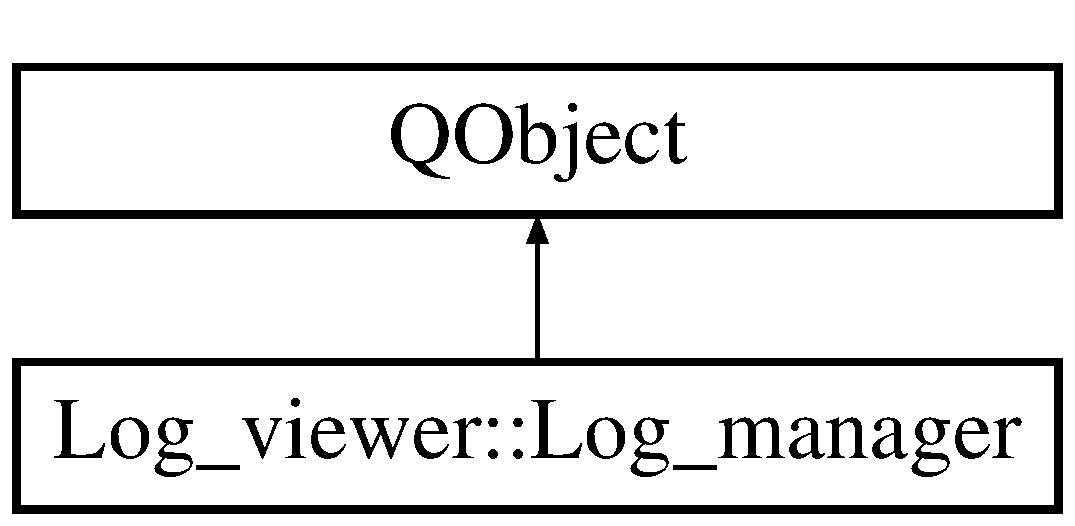
\includegraphics[height=2.000000cm]{class_log__viewer_1_1_log__manager}
\end{center}
\end{figure}
\subsection*{Signals}
\begin{DoxyCompactItemize}
\item 
\hypertarget{class_log__viewer_1_1_log__manager_a66a8c749e6339ba1582a954896a264cc}{void {\bfseries client\-\_\-connected} (const Q\-String \&client\-\_\-address)}\label{class_log__viewer_1_1_log__manager_a66a8c749e6339ba1582a954896a264cc}

\item 
\hypertarget{class_log__viewer_1_1_log__manager_a341b5a25f249c3c9f5c52334b0752cd0}{void {\bfseries client\-\_\-disconnected} (const Q\-String \&client\-\_\-address)}\label{class_log__viewer_1_1_log__manager_a341b5a25f249c3c9f5c52334b0752cd0}

\item 
\hypertarget{class_log__viewer_1_1_log__manager_a43d2039d47502f27419827f1f60b6357}{void {\bfseries server\-\_\-listening} (bool listening)}\label{class_log__viewer_1_1_log__manager_a43d2039d47502f27419827f1f60b6357}

\item 
\hypertarget{class_log__viewer_1_1_log__manager_ab8995449750d2e770f4685771cf04037}{void {\bfseries file\-\_\-opened} (const Q\-String \&file)}\label{class_log__viewer_1_1_log__manager_ab8995449750d2e770f4685771cf04037}

\item 
\hypertarget{class_log__viewer_1_1_log__manager_ab7889c2b1add24d41836163ce6ca647e}{void {\bfseries error} (const Q\-String \&text)}\label{class_log__viewer_1_1_log__manager_ab7889c2b1add24d41836163ce6ca647e}

\item 
\hypertarget{class_log__viewer_1_1_log__manager_a40988e354e6cdc17e232efb579f359b3}{void {\bfseries tail\-\_\-cleared} ()}\label{class_log__viewer_1_1_log__manager_a40988e354e6cdc17e232efb579f359b3}

\item 
\hypertarget{class_log__viewer_1_1_log__manager_a053a5058cb93bcb16b39d1967dbfc832}{void {\bfseries log\-\_\-items\-\_\-empty} ()}\label{class_log__viewer_1_1_log__manager_a053a5058cb93bcb16b39d1967dbfc832}

\item 
\hypertarget{class_log__viewer_1_1_log__manager_a2aec40a074ee9eb6e78c2de0a8b157cb}{void {\bfseries log\-\_\-items\-\_\-not\-\_\-empty} ()}\label{class_log__viewer_1_1_log__manager_a2aec40a074ee9eb6e78c2de0a8b157cb}

\item 
\hypertarget{class_log__viewer_1_1_log__manager_a1e164573afd5549d59b1c699cea9326e}{void {\bfseries log\-\_\-format\-\_\-selected} (const Q\-String \&format)}\label{class_log__viewer_1_1_log__manager_a1e164573afd5549d59b1c699cea9326e}

\item 
\hypertarget{class_log__viewer_1_1_log__manager_acf20aeabbd34f843afae11284c23cb28}{void {\bfseries log\-\_\-proxy\-\_\-filter\-\_\-cleared} ()}\label{class_log__viewer_1_1_log__manager_acf20aeabbd34f843afae11284c23cb28}

\item 
\hypertarget{class_log__viewer_1_1_log__manager_a09689826638db38ec0f7f667b24667c8}{void {\bfseries ftp\-\_\-file\-\_\-downloaded} (const Q\-String \&file\-\_\-name)}\label{class_log__viewer_1_1_log__manager_a09689826638db38ec0f7f667b24667c8}

\end{DoxyCompactItemize}
\subsection*{Public Member Functions}
\begin{DoxyCompactItemize}
\item 
\hypertarget{class_log__viewer_1_1_log__manager_a6f6520f45fed69e1d5533cc712897cd5}{bool {\bfseries listen} (int port)}\label{class_log__viewer_1_1_log__manager_a6f6520f45fed69e1d5533cc712897cd5}

\item 
\hypertarget{class_log__viewer_1_1_log__manager_a52253723b1a1b37ab965d13b3348c9f1}{void {\bfseries close} ()}\label{class_log__viewer_1_1_log__manager_a52253723b1a1b37ab965d13b3348c9f1}

\item 
\hypertarget{class_log__viewer_1_1_log__manager_a4a813b21a06d0d61ecf47bf2ae0bc330}{void {\bfseries open\-\_\-log\-\_\-files} (const Q\-String\-List \&files)}\label{class_log__viewer_1_1_log__manager_a4a813b21a06d0d61ecf47bf2ae0bc330}

\item 
\hypertarget{class_log__viewer_1_1_log__manager_a6bf5991ace8b11c7d696ebc44322ddaf}{void {\bfseries open\-\_\-log} (const Q\-String \&file)}\label{class_log__viewer_1_1_log__manager_a6bf5991ace8b11c7d696ebc44322ddaf}

\item 
\hypertarget{class_log__viewer_1_1_log__manager_ae45a5b9122de8b567c25b76886727353}{void {\bfseries open\-\_\-log\-\_\-from\-\_\-clipboard} ()}\label{class_log__viewer_1_1_log__manager_ae45a5b9122de8b567c25b76886727353}

\item 
\hypertarget{class_log__viewer_1_1_log__manager_ad3101cedf680375523feebd724fb4c32}{void {\bfseries open\-\_\-ftp} (const Q\-String \&host, int port, const Q\-String \&user\-Name, const Q\-String \&password)}\label{class_log__viewer_1_1_log__manager_ad3101cedf680375523feebd724fb4c32}

\item 
\hypertarget{class_log__viewer_1_1_log__manager_a5d5f726f6a79d7ce1946af06afe2016b}{void {\bfseries apply\-\_\-filter} (const Q\-String \&text, const Q\-String \&file, const Q\-String \&module, const Q\-String \&index)}\label{class_log__viewer_1_1_log__manager_a5d5f726f6a79d7ce1946af06afe2016b}

\item 
\hypertarget{class_log__viewer_1_1_log__manager_ae495cc66ef73e09d049f14daea1c8c49}{void {\bfseries clear\-\_\-filter} ()}\label{class_log__viewer_1_1_log__manager_ae495cc66ef73e09d049f14daea1c8c49}

\item 
\hypertarget{class_log__viewer_1_1_log__manager_ad4e708d4dd51d2d5b99db98256065049}{void {\bfseries tail\-\_\-current\-\_\-file} ()}\label{class_log__viewer_1_1_log__manager_ad4e708d4dd51d2d5b99db98256065049}

\item 
\hypertarget{class_log__viewer_1_1_log__manager_ae5f7368756b825bb8a5c5e6e95447492}{void {\bfseries clear\-\_\-tail} ()}\label{class_log__viewer_1_1_log__manager_ae5f7368756b825bb8a5c5e6e95447492}

\item 
\hypertarget{class_log__viewer_1_1_log__manager_ac50136b21ddddda051a8a2c5f1fb119d}{void {\bfseries clear\-\_\-log\-\_\-items} ()}\label{class_log__viewer_1_1_log__manager_ac50136b21ddddda051a8a2c5f1fb119d}

\item 
\hypertarget{class_log__viewer_1_1_log__manager_a89032a90f8e174bf4e05692529243a65}{\hyperlink{class_log__viewer_1_1_log__items__model}{Log\-\_\-items\-\_\-model} $\ast$ {\bfseries log\-\_\-items\-\_\-model} () const }\label{class_log__viewer_1_1_log__manager_a89032a90f8e174bf4e05692529243a65}

\item 
\hypertarget{class_log__viewer_1_1_log__manager_a175cb3f91bbc5ba72db76e0fadfa1333}{\hyperlink{class_log__viewer_1_1ftp__files__model}{ftp\-\_\-files\-\_\-model} $\ast$ {\bfseries ftp\-\_\-model} () const }\label{class_log__viewer_1_1_log__manager_a175cb3f91bbc5ba72db76e0fadfa1333}

\item 
\hypertarget{class_log__viewer_1_1_log__manager_a10c36541f43e869bdd236ee0b9314dc4}{\hyperlink{class_log__viewer_1_1_clients__model}{Clients\-\_\-model} $\ast$ {\bfseries clients\-\_\-model} () const }\label{class_log__viewer_1_1_log__manager_a10c36541f43e869bdd236ee0b9314dc4}

\item 
\hypertarget{class_log__viewer_1_1_log__manager_a604214baff8422513b56b9d250021fc9}{\hyperlink{class_log__viewer_1_1_log__filter__proxy__model}{Log\-\_\-filter\-\_\-proxy\-\_\-model} $\ast$ {\bfseries log\-\_\-filter\-\_\-proxy\-\_\-model} () const }\label{class_log__viewer_1_1_log__manager_a604214baff8422513b56b9d250021fc9}

\item 
\hypertarget{class_log__viewer_1_1_log__manager_a5679b9477da66227847ad81996184c57}{\hyperlink{class_log__viewer_1_1_file__neighbor__model}{File\-\_\-neighbor\-\_\-model} $\ast$ {\bfseries file\-\_\-neighbor\-\_\-model} () const }\label{class_log__viewer_1_1_log__manager_a5679b9477da66227847ad81996184c57}

\item 
\hypertarget{class_log__viewer_1_1_log__manager_a0fef80e0e439fab3a445cb53a490764f}{int {\bfseries get\-\_\-port} ()}\label{class_log__viewer_1_1_log__manager_a0fef80e0e439fab3a445cb53a490764f}

\item 
\hypertarget{class_log__viewer_1_1_log__manager_a6d5a74cbe0295491727a1129c3b50233}{Q\-String {\bfseries get\-\_\-error} ()}\label{class_log__viewer_1_1_log__manager_a6d5a74cbe0295491727a1129c3b50233}

\item 
\hypertarget{class_log__viewer_1_1_log__manager_a5be7c479f5f3acb3ce3739b24200e3a2}{Q\-String {\bfseries get\-\_\-current\-\_\-file} ()}\label{class_log__viewer_1_1_log__manager_a5be7c479f5f3acb3ce3739b24200e3a2}

\end{DoxyCompactItemize}
\subsection*{Static Public Attributes}
\begin{DoxyCompactItemize}
\item 
\hypertarget{class_log__viewer_1_1_log__manager_a7160fd218229d2b36bb3591c978e2eee}{static \hyperlink{class_log__viewer_1_1_log__manager}{Log\-\_\-manager} $\ast$ {\bfseries instance} = \&\hyperlink{class_singleton}{Singleton}$<$\hyperlink{class_log__viewer_1_1_log__manager}{Log\-\_\-manager}$>$\-::Instance()}\label{class_log__viewer_1_1_log__manager_a7160fd218229d2b36bb3591c978e2eee}

\end{DoxyCompactItemize}


The documentation for this class was generated from the following files\-:\begin{DoxyCompactItemize}
\item 
log\-\_\-manager.\-h\item 
log\-\_\-manager.\-cpp\end{DoxyCompactItemize}

\hypertarget{class_log__table__view}{\section{Log\-\_\-table\-\_\-view Class Reference}
\label{class_log__table__view}\index{Log\-\_\-table\-\_\-view@{Log\-\_\-table\-\_\-view}}
}
Inheritance diagram for Log\-\_\-table\-\_\-view\-:\begin{figure}[H]
\begin{center}
\leavevmode
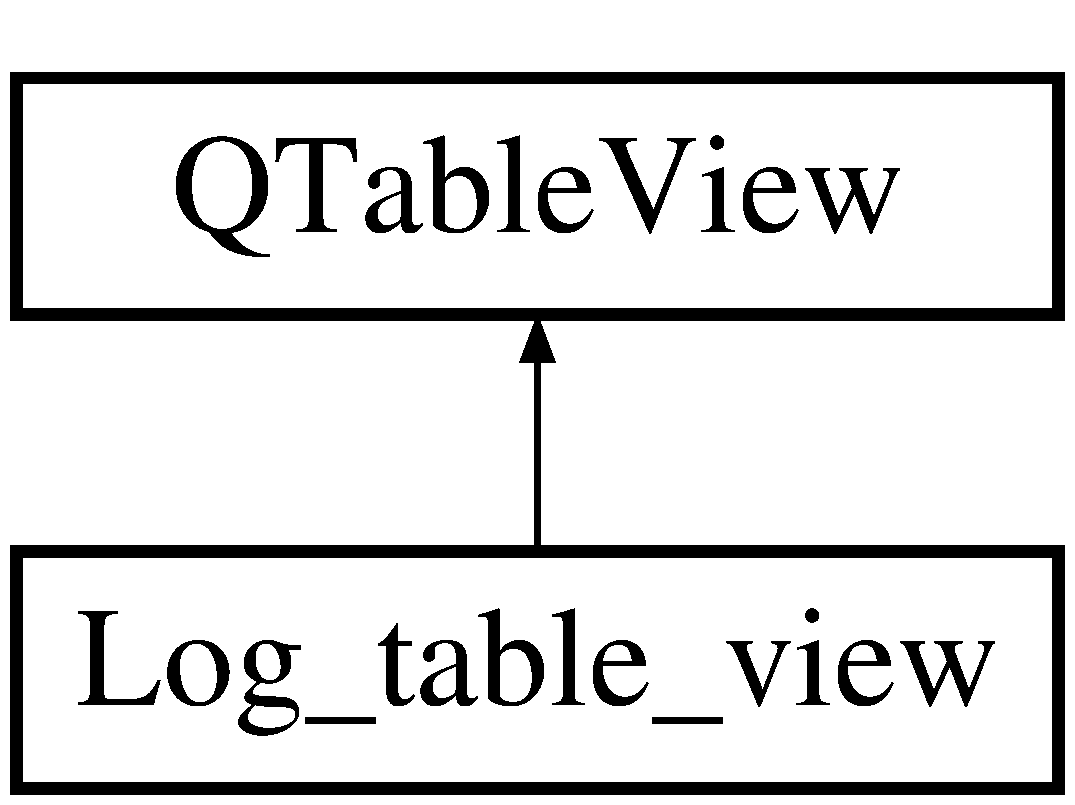
\includegraphics[height=2.000000cm]{class_log__table__view}
\end{center}
\end{figure}
\subsection*{Public Slots}
\begin{DoxyCompactItemize}
\item 
\hypertarget{class_log__table__view_ab2a92cf274fb22465da37f683e67c90b}{void {\bfseries on\-\_\-scroll\-\_\-value\-Changed} (int)}\label{class_log__table__view_ab2a92cf274fb22465da37f683e67c90b}

\item 
\hypertarget{class_log__table__view_aad910b1f34b59b2a1e93ad5b4178733e}{void {\bfseries rows\-Inserted} (const Q\-Model\-Index \&, int, int)}\label{class_log__table__view_aad910b1f34b59b2a1e93ad5b4178733e}

\end{DoxyCompactItemize}
\subsection*{Signals}
\begin{DoxyCompactItemize}
\item 
\hypertarget{class_log__table__view_aa0994c349e5e7059f2f2a31da6222088}{void {\bfseries files\-\_\-dropped} (const Q\-String\-List \&files)}\label{class_log__table__view_aa0994c349e5e7059f2f2a31da6222088}

\item 
\hypertarget{class_log__table__view_a2b269c4fe6915b89410b7aff98addf84}{void {\bfseries enable\-\_\-scroll\-\_\-lock} (bool enable)}\label{class_log__table__view_a2b269c4fe6915b89410b7aff98addf84}

\item 
\hypertarget{class_log__table__view_ac21ba7d1330fef6e8d296152c3d4e51a}{void {\bfseries selected\-\_\-row} (const Q\-String \&row, const Q\-String \&text, const Q\-String \&type, const Q\-String \&file, const Q\-String \&line, const Q\-String \&origin)}\label{class_log__table__view_ac21ba7d1330fef6e8d296152c3d4e51a}

\end{DoxyCompactItemize}
\subsection*{Public Member Functions}
\begin{DoxyCompactItemize}
\item 
\hypertarget{class_log__table__view_a68302857c6f515f9153f6d31398d6afd}{{\bfseries Log\-\_\-table\-\_\-view} (Q\-Widget $\ast$parent=0)}\label{class_log__table__view_a68302857c6f515f9153f6d31398d6afd}

\item 
\hypertarget{class_log__table__view_aefec5bdac7b0b9e0f8f8e93bfa6dec84}{void {\bfseries set\-Model} (Q\-Abstract\-Item\-Model $\ast$model)}\label{class_log__table__view_aefec5bdac7b0b9e0f8f8e93bfa6dec84}

\item 
\hypertarget{class_log__table__view_a70b87261b61a438170e5d902926a4c38}{void {\bfseries set\-Auto\-Scrolling} (bool enable)}\label{class_log__table__view_a70b87261b61a438170e5d902926a4c38}

\item 
\hypertarget{class_log__table__view_a513c602f0f6b9b3781d9f9ec2b0b3c15}{bool {\bfseries auto\-Scrolling} ()}\label{class_log__table__view_a513c602f0f6b9b3781d9f9ec2b0b3c15}

\end{DoxyCompactItemize}
\subsection*{Protected Member Functions}
\begin{DoxyCompactItemize}
\item 
\hypertarget{class_log__table__view_a1526150b50bdf49505c9d9652ac2947d}{void {\bfseries drag\-Enter\-Event} (Q\-Drag\-Enter\-Event $\ast$event)}\label{class_log__table__view_a1526150b50bdf49505c9d9652ac2947d}

\item 
\hypertarget{class_log__table__view_a9d378da78bcfa9cfc5e124d47a340e73}{void {\bfseries drag\-Move\-Event} (Q\-Drag\-Move\-Event $\ast$event)}\label{class_log__table__view_a9d378da78bcfa9cfc5e124d47a340e73}

\item 
\hypertarget{class_log__table__view_ae98dec66199e645f9022c1925543bf8f}{void {\bfseries drag\-Leave\-Event} (Q\-Drag\-Leave\-Event $\ast$event)}\label{class_log__table__view_ae98dec66199e645f9022c1925543bf8f}

\item 
\hypertarget{class_log__table__view_a6ad378c737e744cb5517ae3932190d78}{void {\bfseries drop\-Event} (Q\-Drop\-Event $\ast$event)}\label{class_log__table__view_a6ad378c737e744cb5517ae3932190d78}

\item 
\hypertarget{class_log__table__view_adcb2fff0ead391c99f19bc9eb7ae96a0}{void {\bfseries current\-Changed} (const Q\-Model\-Index \&current, const Q\-Model\-Index \&previous)}\label{class_log__table__view_adcb2fff0ead391c99f19bc9eb7ae96a0}

\end{DoxyCompactItemize}


The documentation for this class was generated from the following files\-:\begin{DoxyCompactItemize}
\item 
log\-\_\-table\-\_\-view.\-h\item 
log\-\_\-table\-\_\-view.\-cpp\end{DoxyCompactItemize}

\hypertarget{class_main__window}{\section{Main\-\_\-window Class Reference}
\label{class_main__window}\index{Main\-\_\-window@{Main\-\_\-window}}
}
Inheritance diagram for Main\-\_\-window\-:\begin{figure}[H]
\begin{center}
\leavevmode
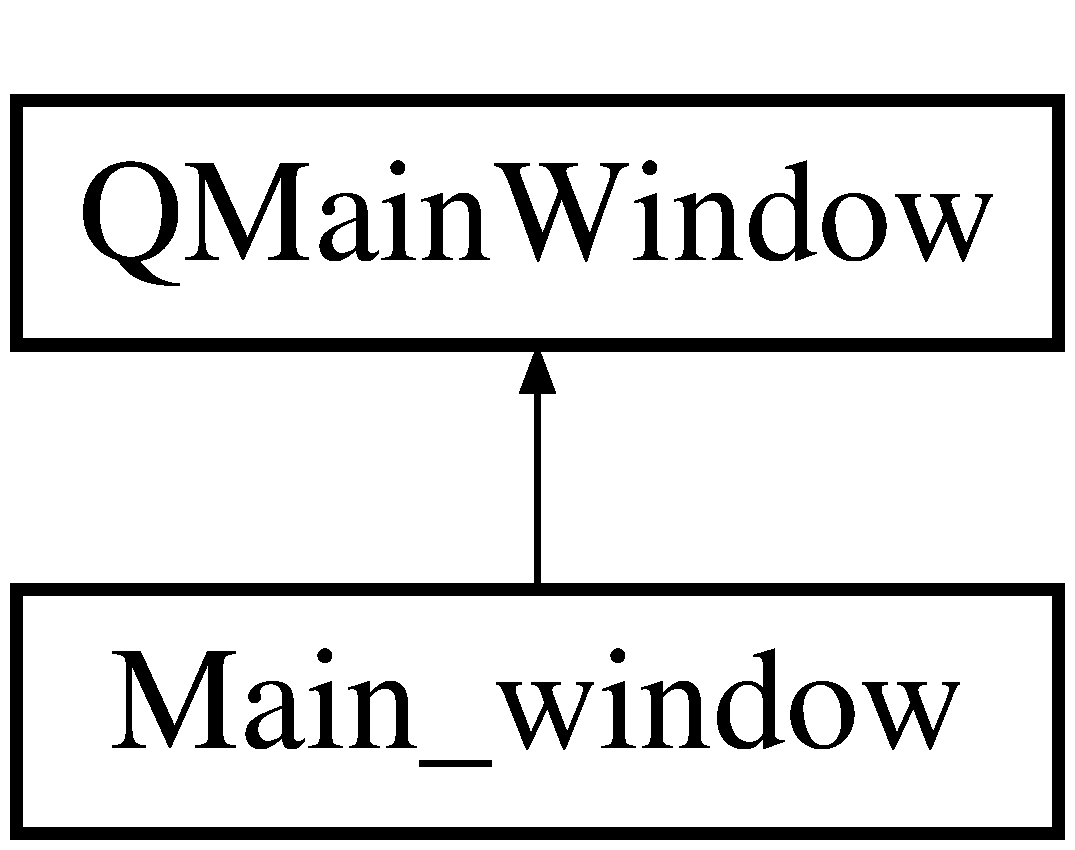
\includegraphics[height=2.000000cm]{class_main__window}
\end{center}
\end{figure}
\subsection*{Public Member Functions}
\begin{DoxyCompactItemize}
\item 
\hypertarget{class_main__window_a6fc238fd46eac0aef63bbaec7eddda02}{{\bfseries Main\-\_\-window} (Q\-Widget $\ast$parent=0)}\label{class_main__window_a6fc238fd46eac0aef63bbaec7eddda02}

\end{DoxyCompactItemize}


The documentation for this class was generated from the following files\-:\begin{DoxyCompactItemize}
\item 
main\-\_\-window.\-h\item 
main\-\_\-window.\-cpp\end{DoxyCompactItemize}

\hypertarget{struct_log__viewer_1_1_n_r_g__legacy__log__format}{\section{Log\-\_\-viewer\-:\-:N\-R\-G\-\_\-legacy\-\_\-log\-\_\-format Struct Reference}
\label{struct_log__viewer_1_1_n_r_g__legacy__log__format}\index{Log\-\_\-viewer\-::\-N\-R\-G\-\_\-legacy\-\_\-log\-\_\-format@{Log\-\_\-viewer\-::\-N\-R\-G\-\_\-legacy\-\_\-log\-\_\-format}}
}
Inheritance diagram for Log\-\_\-viewer\-:\-:N\-R\-G\-\_\-legacy\-\_\-log\-\_\-format\-:\begin{figure}[H]
\begin{center}
\leavevmode
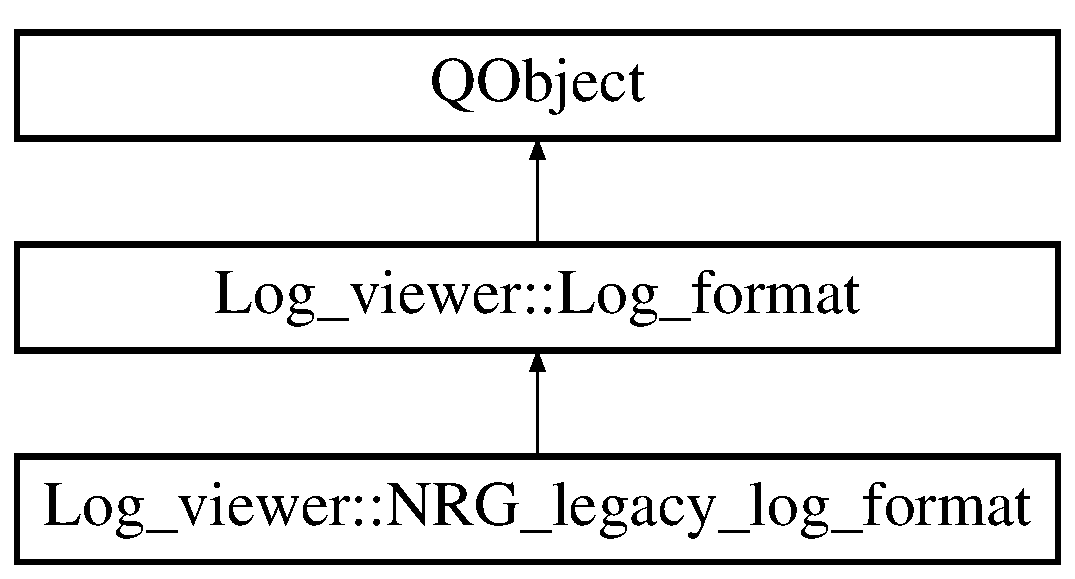
\includegraphics[height=3.000000cm]{struct_log__viewer_1_1_n_r_g__legacy__log__format}
\end{center}
\end{figure}
\subsection*{Public Member Functions}
\begin{DoxyCompactItemize}
\item 
\hypertarget{struct_log__viewer_1_1_n_r_g__legacy__log__format_a91653c6cc26f971003be1c442bdba465}{{\bfseries N\-R\-G\-\_\-legacy\-\_\-log\-\_\-format} (const Q\-String origin, Q\-Object $\ast$parent=0)}\label{struct_log__viewer_1_1_n_r_g__legacy__log__format_a91653c6cc26f971003be1c442bdba465}

\item 
bool \hyperlink{struct_log__viewer_1_1_n_r_g__legacy__log__format_a47061fc90c8b3bb06ee9599f13747442}{match} (const Q\-String first\-\_\-line) const 
\item 
\hypertarget{struct_log__viewer_1_1_n_r_g__legacy__log__format_a41fdb2fb07842f15b37e45b56c3ad88a}{Q\-String {\bfseries get\-\_\-start\-\_\-seq} () const }\label{struct_log__viewer_1_1_n_r_g__legacy__log__format_a41fdb2fb07842f15b37e45b56c3ad88a}

\item 
\hypertarget{struct_log__viewer_1_1_n_r_g__legacy__log__format_a829b88dca1607372247e95668fc9bb31}{Q\-String {\bfseries get\-\_\-stop\-\_\-seq} () const }\label{struct_log__viewer_1_1_n_r_g__legacy__log__format_a829b88dca1607372247e95668fc9bb31}

\item 
\hypertarget{struct_log__viewer_1_1_n_r_g__legacy__log__format_a697fbc75b7bcbdf0aea8433eb060f627}{Q\-String {\bfseries get\-\_\-description} () const }\label{struct_log__viewer_1_1_n_r_g__legacy__log__format_a697fbc75b7bcbdf0aea8433eb060f627}

\item 
\hypertarget{struct_log__viewer_1_1_n_r_g__legacy__log__format_a08649850c6b2fc380da04beb992d6e3a}{Q\-String {\bfseries get\-\_\-origin} () const }\label{struct_log__viewer_1_1_n_r_g__legacy__log__format_a08649850c6b2fc380da04beb992d6e3a}

\item 
\hypertarget{struct_log__viewer_1_1_n_r_g__legacy__log__format_ab8c3dc27076d4143ba112aec2d30ed5e}{Log\-\_\-columns {\bfseries get\-\_\-columns} () const }\label{struct_log__viewer_1_1_n_r_g__legacy__log__format_ab8c3dc27076d4143ba112aec2d30ed5e}

\end{DoxyCompactItemize}
\subsection*{Additional Inherited Members}


\subsection{Member Function Documentation}
\hypertarget{struct_log__viewer_1_1_n_r_g__legacy__log__format_a47061fc90c8b3bb06ee9599f13747442}{\index{Log\-\_\-viewer\-::\-N\-R\-G\-\_\-legacy\-\_\-log\-\_\-format@{Log\-\_\-viewer\-::\-N\-R\-G\-\_\-legacy\-\_\-log\-\_\-format}!match@{match}}
\index{match@{match}!Log_viewer::NRG_legacy_log_format@{Log\-\_\-viewer\-::\-N\-R\-G\-\_\-legacy\-\_\-log\-\_\-format}}
\subsubsection[{match}]{\setlength{\rightskip}{0pt plus 5cm}bool Log\-\_\-viewer\-::\-N\-R\-G\-\_\-legacy\-\_\-log\-\_\-format\-::match (
\begin{DoxyParamCaption}
\item[{const Q\-String}]{first\-\_\-line}
\end{DoxyParamCaption}
) const\hspace{0.3cm}{\ttfamily [inline]}, {\ttfamily [virtual]}}}\label{struct_log__viewer_1_1_n_r_g__legacy__log__format_a47061fc90c8b3bb06ee9599f13747442}
This method returns true if we can match the passed line.

A regular expression is used to match the first\-\_\-line. N\-R\-G lecacy format expects the line to start with a date formated like this\-: \begin{DoxyParagraph}{2010-\/09-\/08 12\-:06\-:12,079}

\end{DoxyParagraph}
and shall be followed by a S\-P\-A\-C\-E and a pipe char after the date. 

Implements \hyperlink{class_log__viewer_1_1_log__format}{Log\-\_\-viewer\-::\-Log\-\_\-format}.



The documentation for this struct was generated from the following file\-:\begin{DoxyCompactItemize}
\item 
nrg\-\_\-legacy\-\_\-log\-\_\-format.\-h\end{DoxyCompactItemize}

\hypertarget{class_log__viewer_1_1_n_r_g__legacy__log__item}{\section{Log\-\_\-viewer\-:\-:N\-R\-G\-\_\-legacy\-\_\-log\-\_\-item Class Reference}
\label{class_log__viewer_1_1_n_r_g__legacy__log__item}\index{Log\-\_\-viewer\-::\-N\-R\-G\-\_\-legacy\-\_\-log\-\_\-item@{Log\-\_\-viewer\-::\-N\-R\-G\-\_\-legacy\-\_\-log\-\_\-item}}
}
Inheritance diagram for Log\-\_\-viewer\-:\-:N\-R\-G\-\_\-legacy\-\_\-log\-\_\-item\-:\begin{figure}[H]
\begin{center}
\leavevmode
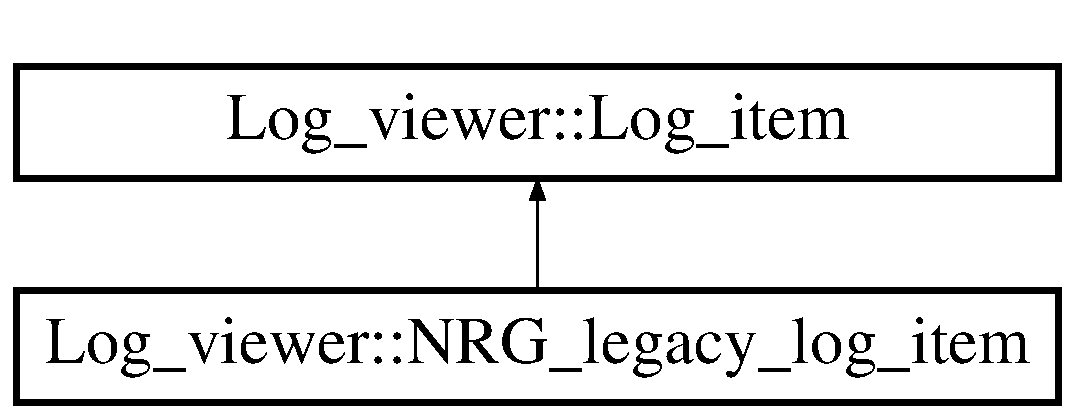
\includegraphics[height=2.000000cm]{class_log__viewer_1_1_n_r_g__legacy__log__item}
\end{center}
\end{figure}
\subsection*{Public Member Functions}
\begin{DoxyCompactItemize}
\item 
\hypertarget{class_log__viewer_1_1_n_r_g__legacy__log__item_a45bc36e7f11f11f7159f37008ff4791c}{{\bfseries N\-R\-G\-\_\-legacy\-\_\-log\-\_\-item} (const Q\-String \&value, const Q\-String \&separator, const Q\-String \&origin)}\label{class_log__viewer_1_1_n_r_g__legacy__log__item_a45bc36e7f11f11f7159f37008ff4791c}

\end{DoxyCompactItemize}
\subsection*{Protected Member Functions}
\begin{DoxyCompactItemize}
\item 
\hypertarget{class_log__viewer_1_1_n_r_g__legacy__log__item_a6485c7e03d5d0db58fddc76dbb5c190f}{Log\-\_\-type {\bfseries Log\-\_\-type\-\_\-from\-\_\-string} (const Q\-String value)}\label{class_log__viewer_1_1_n_r_g__legacy__log__item_a6485c7e03d5d0db58fddc76dbb5c190f}

\end{DoxyCompactItemize}
\subsection*{Additional Inherited Members}


The documentation for this class was generated from the following files\-:\begin{DoxyCompactItemize}
\item 
nrg\-\_\-legacy\-\_\-log\-\_\-item.\-h\item 
nrg\-\_\-legacy\-\_\-log\-\_\-item.\-cpp\end{DoxyCompactItemize}

\hypertarget{struct_log__viewer_1_1_n_r_g__log__format}{\section{Log\-\_\-viewer\-:\-:N\-R\-G\-\_\-log\-\_\-format Struct Reference}
\label{struct_log__viewer_1_1_n_r_g__log__format}\index{Log\-\_\-viewer\-::\-N\-R\-G\-\_\-log\-\_\-format@{Log\-\_\-viewer\-::\-N\-R\-G\-\_\-log\-\_\-format}}
}
Inheritance diagram for Log\-\_\-viewer\-:\-:N\-R\-G\-\_\-log\-\_\-format\-:\begin{figure}[H]
\begin{center}
\leavevmode
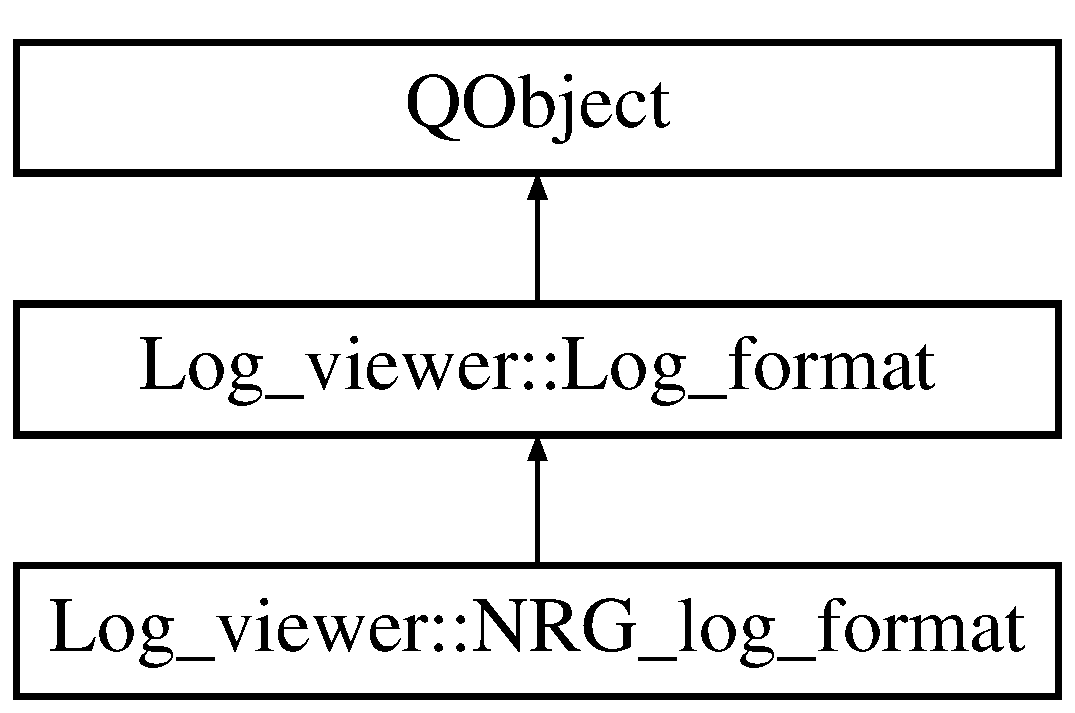
\includegraphics[height=3.000000cm]{struct_log__viewer_1_1_n_r_g__log__format}
\end{center}
\end{figure}
\subsection*{Public Member Functions}
\begin{DoxyCompactItemize}
\item 
\hypertarget{struct_log__viewer_1_1_n_r_g__log__format_aa1c60c8059b20a6f9c958450e9f19a50}{{\bfseries N\-R\-G\-\_\-log\-\_\-format} (const Q\-String origin, Q\-Object $\ast$parent=0)}\label{struct_log__viewer_1_1_n_r_g__log__format_aa1c60c8059b20a6f9c958450e9f19a50}

\item 
bool \hyperlink{struct_log__viewer_1_1_n_r_g__log__format_a32d9e5e346b1fabce16b8c680de2d4de}{match} (const Q\-String first\-\_\-line) const 
\item 
\hypertarget{struct_log__viewer_1_1_n_r_g__log__format_a77b2f35c1b5cdd36db1e2c15ef7e97a2}{Q\-String {\bfseries get\-\_\-start\-\_\-seq} () const }\label{struct_log__viewer_1_1_n_r_g__log__format_a77b2f35c1b5cdd36db1e2c15ef7e97a2}

\item 
\hypertarget{struct_log__viewer_1_1_n_r_g__log__format_a51cc946fb782eeb6bed0a8230d6dc634}{Q\-String {\bfseries get\-\_\-stop\-\_\-seq} () const }\label{struct_log__viewer_1_1_n_r_g__log__format_a51cc946fb782eeb6bed0a8230d6dc634}

\item 
\hypertarget{struct_log__viewer_1_1_n_r_g__log__format_a655a48f686373f89b3ea4814a6cf7d49}{Q\-String {\bfseries get\-\_\-description} () const }\label{struct_log__viewer_1_1_n_r_g__log__format_a655a48f686373f89b3ea4814a6cf7d49}

\item 
\hypertarget{struct_log__viewer_1_1_n_r_g__log__format_ab5f59f53dc62cceb39bfd661ca702971}{Q\-String {\bfseries get\-\_\-origin} () const }\label{struct_log__viewer_1_1_n_r_g__log__format_ab5f59f53dc62cceb39bfd661ca702971}

\item 
\hypertarget{struct_log__viewer_1_1_n_r_g__log__format_a3b85740cec7a649f3c053c1ce6e3246d}{Log\-\_\-columns {\bfseries get\-\_\-columns} () const }\label{struct_log__viewer_1_1_n_r_g__log__format_a3b85740cec7a649f3c053c1ce6e3246d}

\end{DoxyCompactItemize}
\subsection*{Additional Inherited Members}


\subsection{Member Function Documentation}
\hypertarget{struct_log__viewer_1_1_n_r_g__log__format_a32d9e5e346b1fabce16b8c680de2d4de}{\index{Log\-\_\-viewer\-::\-N\-R\-G\-\_\-log\-\_\-format@{Log\-\_\-viewer\-::\-N\-R\-G\-\_\-log\-\_\-format}!match@{match}}
\index{match@{match}!Log_viewer::NRG_log_format@{Log\-\_\-viewer\-::\-N\-R\-G\-\_\-log\-\_\-format}}
\subsubsection[{match}]{\setlength{\rightskip}{0pt plus 5cm}bool Log\-\_\-viewer\-::\-N\-R\-G\-\_\-log\-\_\-format\-::match (
\begin{DoxyParamCaption}
\item[{const Q\-String}]{first\-\_\-line}
\end{DoxyParamCaption}
) const\hspace{0.3cm}{\ttfamily [inline]}, {\ttfamily [virtual]}}}\label{struct_log__viewer_1_1_n_r_g__log__format_a32d9e5e346b1fabce16b8c680de2d4de}
This method returns true if we can match the passed line.

A regular expression is used to match the first\-\_\-line. N\-R\-G format expects the line to start with \char`\"{}start of text\char`\"{} 0x02, followed by a date formated like this\-: \begin{DoxyParagraph}{2010-\/09-\/08 12\-:06\-:12,079864}

\end{DoxyParagraph}
and shall be followed by T\-A\-B char after the date. 

Implements \hyperlink{class_log__viewer_1_1_log__format}{Log\-\_\-viewer\-::\-Log\-\_\-format}.



The documentation for this struct was generated from the following file\-:\begin{DoxyCompactItemize}
\item 
nrg\-\_\-log\-\_\-format.\-h\end{DoxyCompactItemize}

\hypertarget{class_log__viewer_1_1_n_r_g__log__item}{\section{Log\-\_\-viewer\-:\-:N\-R\-G\-\_\-log\-\_\-item Class Reference}
\label{class_log__viewer_1_1_n_r_g__log__item}\index{Log\-\_\-viewer\-::\-N\-R\-G\-\_\-log\-\_\-item@{Log\-\_\-viewer\-::\-N\-R\-G\-\_\-log\-\_\-item}}
}
Inheritance diagram for Log\-\_\-viewer\-:\-:N\-R\-G\-\_\-log\-\_\-item\-:\begin{figure}[H]
\begin{center}
\leavevmode
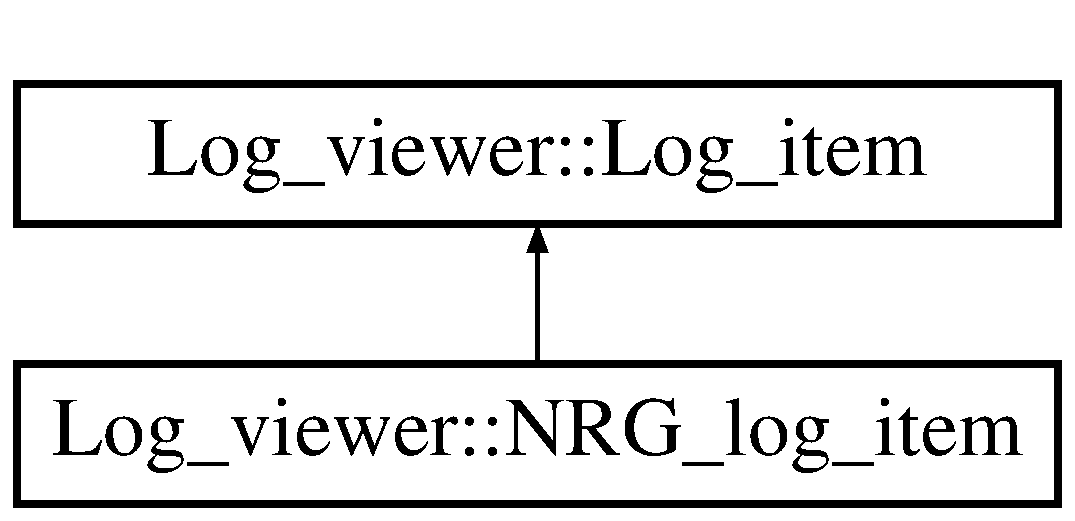
\includegraphics[height=2.000000cm]{class_log__viewer_1_1_n_r_g__log__item}
\end{center}
\end{figure}
\subsection*{Public Member Functions}
\begin{DoxyCompactItemize}
\item 
\hypertarget{class_log__viewer_1_1_n_r_g__log__item_ad0e0673aaa3ef377a481d25d3d5e1ebe}{{\bfseries N\-R\-G\-\_\-log\-\_\-item} (const Q\-String value, const Q\-String separator, const Q\-String origin)}\label{class_log__viewer_1_1_n_r_g__log__item_ad0e0673aaa3ef377a481d25d3d5e1ebe}

\end{DoxyCompactItemize}
\subsection*{Protected Member Functions}
\begin{DoxyCompactItemize}
\item 
\hypertarget{class_log__viewer_1_1_n_r_g__log__item_a65ef836ae997a66077782c95a365260b}{Log\-\_\-type {\bfseries Log\-\_\-type\-\_\-from\-\_\-string} (const Q\-String value)}\label{class_log__viewer_1_1_n_r_g__log__item_a65ef836ae997a66077782c95a365260b}

\end{DoxyCompactItemize}
\subsection*{Additional Inherited Members}


The documentation for this class was generated from the following files\-:\begin{DoxyCompactItemize}
\item 
nrg\-\_\-log\-\_\-item.\-h\item 
nrg\-\_\-log\-\_\-item.\-cpp\end{DoxyCompactItemize}

\hypertarget{class_log__viewer_1_1_plain__text__log__item}{\section{Log\-\_\-viewer\-:\-:Plain\-\_\-text\-\_\-log\-\_\-item Class Reference}
\label{class_log__viewer_1_1_plain__text__log__item}\index{Log\-\_\-viewer\-::\-Plain\-\_\-text\-\_\-log\-\_\-item@{Log\-\_\-viewer\-::\-Plain\-\_\-text\-\_\-log\-\_\-item}}
}
Inheritance diagram for Log\-\_\-viewer\-:\-:Plain\-\_\-text\-\_\-log\-\_\-item\-:\begin{figure}[H]
\begin{center}
\leavevmode
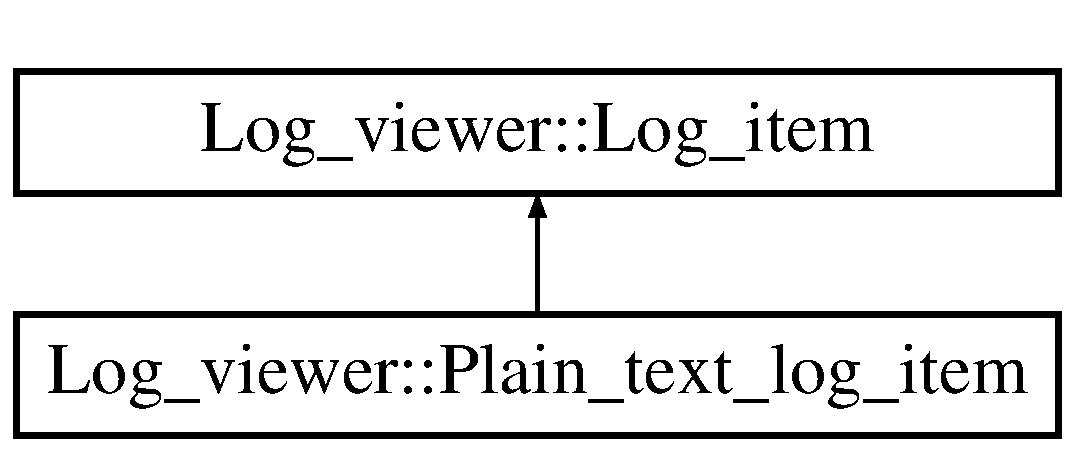
\includegraphics[height=2.000000cm]{class_log__viewer_1_1_plain__text__log__item}
\end{center}
\end{figure}
\subsection*{Public Member Functions}
\begin{DoxyCompactItemize}
\item 
\hypertarget{class_log__viewer_1_1_plain__text__log__item_ab989811bd6b3df0029a04c181befa323}{{\bfseries Plain\-\_\-text\-\_\-log\-\_\-item} (const Q\-String \&value)}\label{class_log__viewer_1_1_plain__text__log__item_ab989811bd6b3df0029a04c181befa323}

\end{DoxyCompactItemize}
\subsection*{Protected Member Functions}
\begin{DoxyCompactItemize}
\item 
\hypertarget{class_log__viewer_1_1_plain__text__log__item_a2f5b569bfdfabd9c4d71f0a1f009de5b}{Log\-\_\-type {\bfseries Log\-\_\-type\-\_\-from\-\_\-string} (const Q\-String)}\label{class_log__viewer_1_1_plain__text__log__item_a2f5b569bfdfabd9c4d71f0a1f009de5b}

\end{DoxyCompactItemize}
\subsection*{Additional Inherited Members}


The documentation for this class was generated from the following files\-:\begin{DoxyCompactItemize}
\item 
plain\-\_\-text\-\_\-log\-\_\-item.\-h\item 
plain\-\_\-text\-\_\-log\-\_\-item.\-cpp\end{DoxyCompactItemize}

\hypertarget{class_singleton}{\section{Singleton$<$ T $>$ Class Template Reference}
\label{class_singleton}\index{Singleton$<$ T $>$@{Singleton$<$ T $>$}}
}
\subsection*{Static Public Member Functions}
\begin{DoxyCompactItemize}
\item 
\hypertarget{class_singleton_a131e87528259529400d58b6df5d9743c}{static T \& {\bfseries Instance} ()}\label{class_singleton_a131e87528259529400d58b6df5d9743c}

\end{DoxyCompactItemize}


The documentation for this class was generated from the following file\-:\begin{DoxyCompactItemize}
\item 
singleton.\-h\end{DoxyCompactItemize}

\hypertarget{class_log__viewer_1_1_start__stop__buffer}{\section{Log\-\_\-viewer\-:\-:Start\-\_\-stop\-\_\-buffer Class Reference}
\label{class_log__viewer_1_1_start__stop__buffer}\index{Log\-\_\-viewer\-::\-Start\-\_\-stop\-\_\-buffer@{Log\-\_\-viewer\-::\-Start\-\_\-stop\-\_\-buffer}}
}
Inheritance diagram for Log\-\_\-viewer\-:\-:Start\-\_\-stop\-\_\-buffer\-:\begin{figure}[H]
\begin{center}
\leavevmode
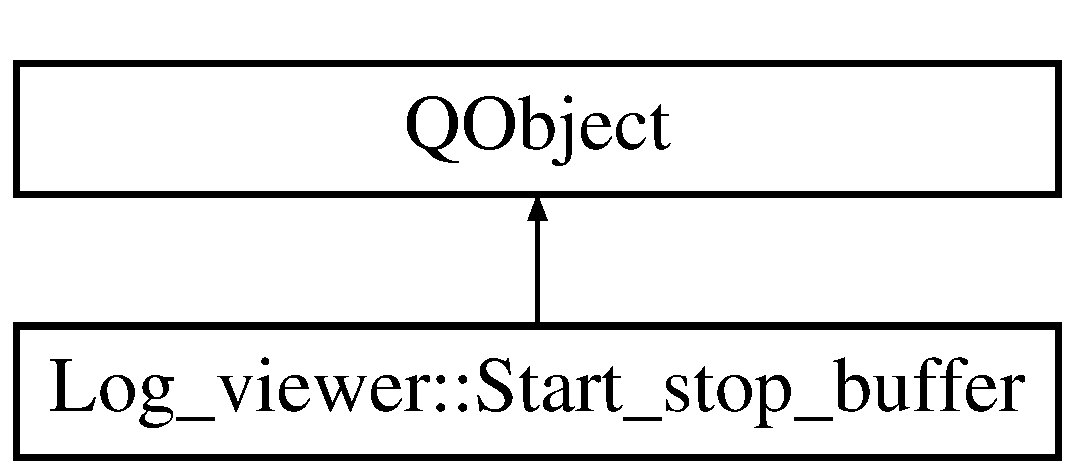
\includegraphics[height=2.000000cm]{class_log__viewer_1_1_start__stop__buffer}
\end{center}
\end{figure}
\subsection*{Signals}
\begin{DoxyCompactItemize}
\item 
\hypertarget{class_log__viewer_1_1_start__stop__buffer_a400dc9ab4a618a67f32d7fe4fed36e91}{void {\bfseries string\-\_\-found} (const Q\-String value)}\label{class_log__viewer_1_1_start__stop__buffer_a400dc9ab4a618a67f32d7fe4fed36e91}

\end{DoxyCompactItemize}
\subsection*{Public Member Functions}
\begin{DoxyCompactItemize}
\item 
\hypertarget{class_log__viewer_1_1_start__stop__buffer_ae5cddbe89a87ad6c06f94e92b4dccb1d}{{\bfseries Start\-\_\-stop\-\_\-buffer} (Q\-Object $\ast$parent)}\label{class_log__viewer_1_1_start__stop__buffer_ae5cddbe89a87ad6c06f94e92b4dccb1d}

\item 
\hypertarget{class_log__viewer_1_1_start__stop__buffer_abdc4d0581880f1fbd39574a6edf4bcf1}{{\bfseries Start\-\_\-stop\-\_\-buffer} (const Q\-String start\-\_\-seq, const Q\-String stop\-\_\-seq)}\label{class_log__viewer_1_1_start__stop__buffer_abdc4d0581880f1fbd39574a6edf4bcf1}

\item 
\hypertarget{class_log__viewer_1_1_start__stop__buffer_aea7fdae2446221e5f425bd1db84c2648}{void {\bfseries set\-\_\-start\-\_\-seq} (const Q\-String value)}\label{class_log__viewer_1_1_start__stop__buffer_aea7fdae2446221e5f425bd1db84c2648}

\item 
\hypertarget{class_log__viewer_1_1_start__stop__buffer_a75a891ba2d32f61c80d778155a60079d}{void {\bfseries set\-\_\-stop\-\_\-seq} (const Q\-String value)}\label{class_log__viewer_1_1_start__stop__buffer_a75a891ba2d32f61c80d778155a60079d}

\item 
\hypertarget{class_log__viewer_1_1_start__stop__buffer_a34a6c39a3a78b7bbc56324d8a9f898f3}{void {\bfseries add} (const Q\-String data)}\label{class_log__viewer_1_1_start__stop__buffer_a34a6c39a3a78b7bbc56324d8a9f898f3}

\end{DoxyCompactItemize}


The documentation for this class was generated from the following files\-:\begin{DoxyCompactItemize}
\item 
start\-\_\-stop\-\_\-buffer.\-h\item 
start\-\_\-stop\-\_\-buffer.\-cpp\end{DoxyCompactItemize}

\hypertarget{class_log__viewer_1_1_tail}{\section{Log\-\_\-viewer\-:\-:Tail Class Reference}
\label{class_log__viewer_1_1_tail}\index{Log\-\_\-viewer\-::\-Tail@{Log\-\_\-viewer\-::\-Tail}}
}
Inheritance diagram for Log\-\_\-viewer\-:\-:Tail\-:\begin{figure}[H]
\begin{center}
\leavevmode
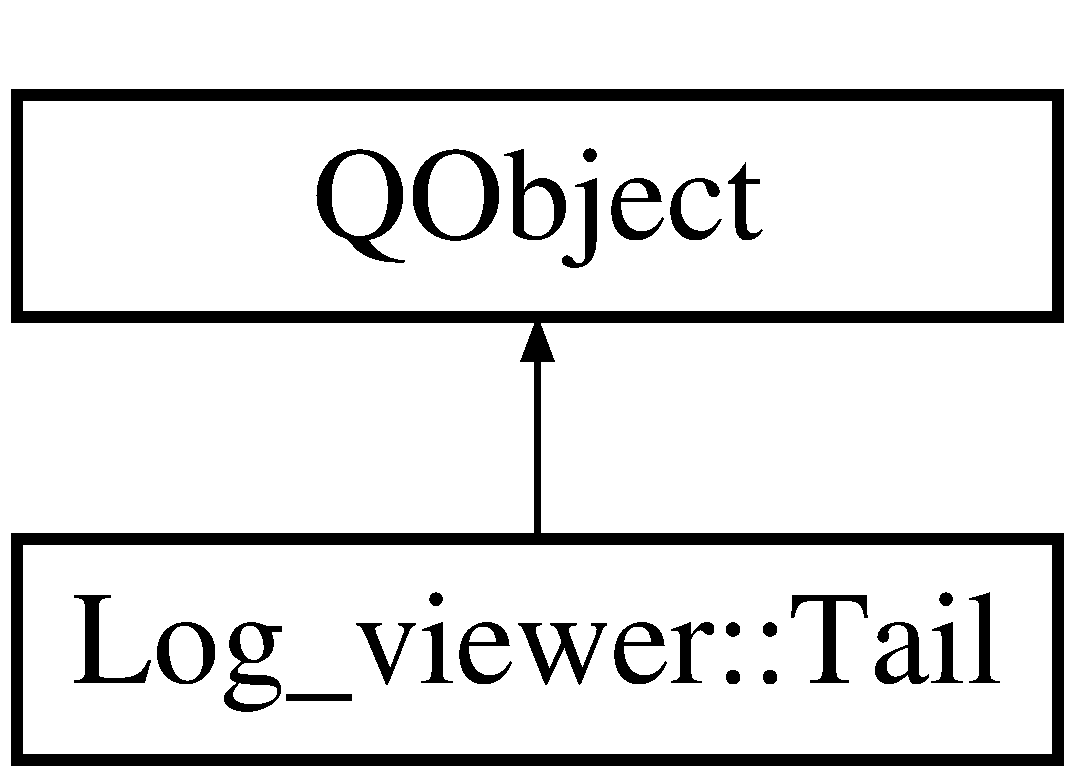
\includegraphics[height=2.000000cm]{class_log__viewer_1_1_tail}
\end{center}
\end{figure}
\subsection*{Signals}
\begin{DoxyCompactItemize}
\item 
\hypertarget{class_log__viewer_1_1_tail_a2ce362f9469de5b705b3960b2ebc833e}{void {\bfseries tail\-\_\-log\-\_\-found} (Q\-Shared\-Pointer$<$ \hyperlink{class_log__viewer_1_1_log__item}{Log\-\_\-item} $>$ item)}\label{class_log__viewer_1_1_tail_a2ce362f9469de5b705b3960b2ebc833e}

\item 
\hypertarget{class_log__viewer_1_1_tail_ab6786e71e42cb38307eeb1dc8cd42568}{void {\bfseries tail\-\_\-empty} ()}\label{class_log__viewer_1_1_tail_ab6786e71e42cb38307eeb1dc8cd42568}

\item 
\hypertarget{class_log__viewer_1_1_tail_ae5ccb520db28b8d0cbdce0058fb02186}{void {\bfseries tail\-\_\-failed} (const Q\-String \&message)}\label{class_log__viewer_1_1_tail_ae5ccb520db28b8d0cbdce0058fb02186}

\end{DoxyCompactItemize}
\subsection*{Public Member Functions}
\begin{DoxyCompactItemize}
\item 
\hypertarget{class_log__viewer_1_1_tail_a2594843c80c46319b34897ffe664fde1}{{\bfseries Tail} (const Q\-String \&file, qint64 file\-\_\-pos, Q\-Shared\-Pointer$<$ \hyperlink{class_log__viewer_1_1_log__format}{Log\-\_\-format} $>$ log\-\_\-format, Q\-Object $\ast$parent=0)}\label{class_log__viewer_1_1_tail_a2594843c80c46319b34897ffe664fde1}

\end{DoxyCompactItemize}


The documentation for this class was generated from the following files\-:\begin{DoxyCompactItemize}
\item 
tail.\-h\item 
tail.\-cpp\end{DoxyCompactItemize}

\hypertarget{struct_log__viewer_1_1_unknown__log__format}{\section{Log\-\_\-viewer\-:\-:Unknown\-\_\-log\-\_\-format Struct Reference}
\label{struct_log__viewer_1_1_unknown__log__format}\index{Log\-\_\-viewer\-::\-Unknown\-\_\-log\-\_\-format@{Log\-\_\-viewer\-::\-Unknown\-\_\-log\-\_\-format}}
}
Inheritance diagram for Log\-\_\-viewer\-:\-:Unknown\-\_\-log\-\_\-format\-:\begin{figure}[H]
\begin{center}
\leavevmode
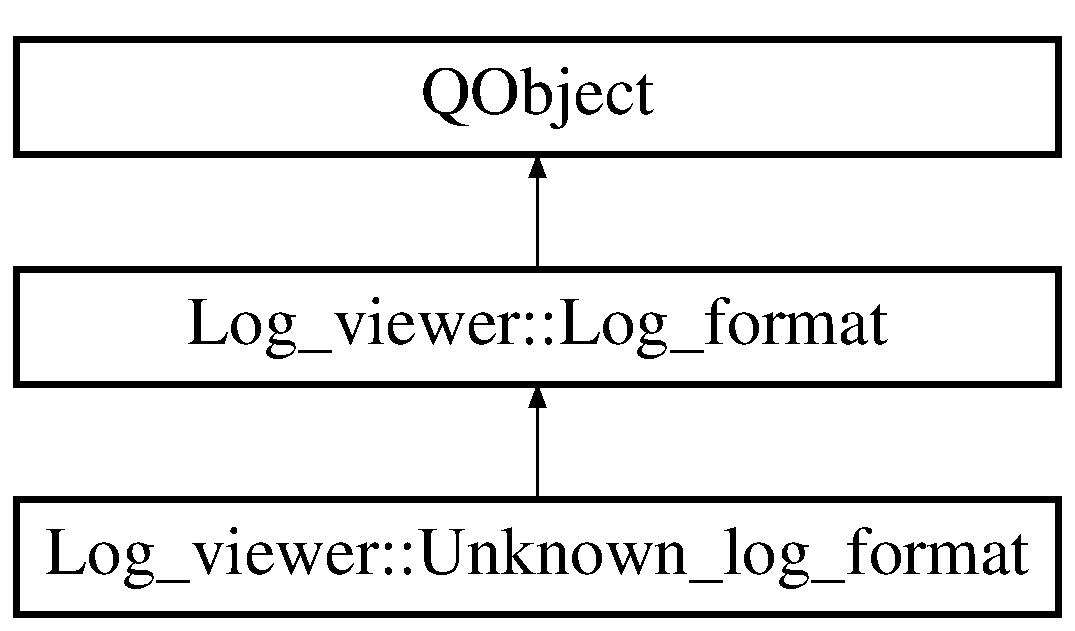
\includegraphics[height=3.000000cm]{struct_log__viewer_1_1_unknown__log__format}
\end{center}
\end{figure}
\subsection*{Public Member Functions}
\begin{DoxyCompactItemize}
\item 
\hypertarget{struct_log__viewer_1_1_unknown__log__format_aad8ef2abb60df94f8c08187580069378}{{\bfseries Unknown\-\_\-log\-\_\-format} (Q\-Object $\ast$parent=0)}\label{struct_log__viewer_1_1_unknown__log__format_aad8ef2abb60df94f8c08187580069378}

\item 
\hypertarget{struct_log__viewer_1_1_unknown__log__format_abf1148548bdeab6abdb08271ca1299fd}{bool {\bfseries match} (const Q\-String) const }\label{struct_log__viewer_1_1_unknown__log__format_abf1148548bdeab6abdb08271ca1299fd}

\item 
\hypertarget{struct_log__viewer_1_1_unknown__log__format_abc19c19826203db3f7f66e12eccbba38}{Q\-String {\bfseries get\-\_\-start\-\_\-seq} () const }\label{struct_log__viewer_1_1_unknown__log__format_abc19c19826203db3f7f66e12eccbba38}

\item 
\hypertarget{struct_log__viewer_1_1_unknown__log__format_a09f98a3a65d8e77bdca6221695192350}{Q\-String {\bfseries get\-\_\-stop\-\_\-seq} () const }\label{struct_log__viewer_1_1_unknown__log__format_a09f98a3a65d8e77bdca6221695192350}

\item 
\hypertarget{struct_log__viewer_1_1_unknown__log__format_a72e95127f494c1a3929616992fe1db87}{Q\-String {\bfseries get\-\_\-description} () const }\label{struct_log__viewer_1_1_unknown__log__format_a72e95127f494c1a3929616992fe1db87}

\item 
\hypertarget{struct_log__viewer_1_1_unknown__log__format_a02e90d395641c589b9d8d4f07e095fbd}{Q\-String {\bfseries get\-\_\-origin} () const }\label{struct_log__viewer_1_1_unknown__log__format_a02e90d395641c589b9d8d4f07e095fbd}

\item 
\hypertarget{struct_log__viewer_1_1_unknown__log__format_ae3d72f0462bbcaecb8d1979db6844427}{Log\-\_\-columns {\bfseries get\-\_\-columns} () const }\label{struct_log__viewer_1_1_unknown__log__format_ae3d72f0462bbcaecb8d1979db6844427}

\end{DoxyCompactItemize}
\subsection*{Additional Inherited Members}


The documentation for this struct was generated from the following file\-:\begin{DoxyCompactItemize}
\item 
unknown\-\_\-log\-\_\-format.\-h\end{DoxyCompactItemize}

%--- End generated contents ---

% Index
\newpage
\phantomsection
\addcontentsline{toc}{part}{Index}
\printindex

\end{document}
